% Основная часть
\section{Аналитическая часть}

\hspace{1.25cm}
В данном разделе будут представлены описание объектов сцены, а также обоснование выбора алгоритмов, которые будут использоваться для визуализации.

\subsection{Описание объектов сцены}

\hspace{1.25cm}
Сцена состоит из различных объектов, включая стены, окна и двери. Каждый объект может быть представлен в виде параллелепипеда с заданными параметрами длины, ширины и высоты. Особое место среди объектов занимает сама сцена -- это плоскость, состоящая из заданного пользователем количества квадратов, размерами которых измеряются следующие объекты и относительно которых задаётся расположение стен, окон и дверей на экране.

\begin{enumerate}
\item Стена -- это параллелепипед с заданными размерами, ограничивающий пространство. Стены могут быть различной толщины и высоты и по разному располагаться на сцене в зависимости от характеристик помещения. Эти объекты используются для формирования границ помещения.

\item Окно -- это плоский объект, встроенный в стену. Его размеры могут варьироваться в зависимости от проекта. Окна также могут быть расположены на разных уровнях стен.

\item Дверь -- это параллелепипед, также встроенный в стену, с возможностью регулирования размера и положения.

\item Источник света -- это точка, расположенная где-то далеко в бесконечности. Он излучает световые лучи во все стороны, что позволяет освещать сцену и создавать тени. Положение источника света можно изменять для достижения различных визуальных эффектов и освещенности объектов сцены.

\item Камера -- представляет собой объект, который может вращаться и рассматривать сцену с разных сторон и расстояний. Камера позволяет настраивать угол обзора, масштаб и положение относительно объектов сцены, что даёт возможность пользователю детально осмотреть помещение.
\end{enumerate}

Эти объекты могут иметь различные параметры, что позволяет создавать уникальные конфигурации помещений, соответствующие потребностям пользователя и требованиям дизайна.



\subsection{Выбор формы задания трёхмерных моделей}

\hspace{1.25cm}
В процессе 3D моделирования создаются геометрические модели, т.е. модели, отражающие геометрические свойства изделий. Различают геометрические модели каркасные (проволочные), поверхностные, объемные (твердотельные).

\begin{enumerate}
\item Каркасная модель представляет форму детали в виде конечного множества линий, лежащих на поверхностях детали. Для каждой линии известны координаты концевых точек и указана их инцидентность рёбрам или поверхностям.

\item Поверхностная модель отображает форму детали с помощью задания ограничивающих её поверхностей, например, в виде совокупности данных о гранях, рёбрах и вершинах. Возможны различные виды задания поверхностей — плоскости, поверхности вращения, линейчатые поверхности.

\item Объёмная модель позволяет представить сложные изделия с обеспечением логической связанности информации, в частности, благодаря введению понятия о материале. В такой модели хранится информация, позволяющая отличать материал от пустоты, при этом пустота может рассматриваться как особый вид материала.~\cite{kgau}
\end{enumerate}

В процессе 3D-моделирования выбор геометрической модели зависит от целей и характеристик задачи. Каркасные модели предоставляют лишь ограниченную информацию о форме объекта, что не всегда подходит для детализированного представления. Объёмные модели дают полное представление о внутреннем содержании, но они требуют значительно больше вычислительных ресурсов для обработки.

В рамках данной работы была выбрана поверхностная модель. Этот выбор обусловлен тем, что поверхностные модели позволяют эффективно представлять форму объекта с помощью ограничивающих его поверхностей, что идеально подходит для визуализации объектов на сцене. Поверхностная модель даёт возможность адекватно отобразить внешний вид объектов (стен, окон, дверей), при этом её использование не требует таких значительных вычислительных затрат, как объёмные модели. Такая модель также достаточно гибка для выполнения операций, связанных с рендерингом и проверкой взаимодействий объектов на сцене.



\subsection{Выбор алгоритма удаления невидимых линий}

\subsubsection{Введение}

\hspace{1.25cm}
Одной из основных задач компьютерной графики является визуализация трёхмерных сцен. Подобные задачи возникают в системах автоматизированного проектирования, пакетах моделирования физических процессов, средствах компьютерной анимации и виртуальной реальности.

При отображении трёхмерной сцены на экране некоторые из объектов сцены могут заслонить другие объекты. Заслонённые части объектов невидимы и не должны рисоваться, или должны рисоваться иначе, чем видимые части, например, пунктиром. Если этого не делать, то изображение будет выглядеть неправильно.

Такие задачи решают с помощью алгоритмов удаления невидимых линий и поверхностей. Если сцена отображается в каркасном виде, линиями, то нужно удалять невидимые линии. Каркасное изображение обычно строится из отрезков – рёбер, и алгоритм должен выделить части отрезков, заслонённых объектами сцены. Если объекты сцены отображаются в виде закрашенных поверхностей, то нужно удалять невидимые части этих поверхностей. Обычно в качестве поверхностей используются выпуклые многоугольники, чаще всего – треугольники.
В курсовой работе необходимо реализовать один из алгоритмов удаления невидимых линий и поверхностей и произвести анализ его производительности. В соответствующих разделах приведены описания основных алгоритмов: Робертса, Варнака, Z-буфера, художника, трассировки лучей, построчного сканирования.

Все алгоритмы удаления невидимых линий и поверхностей можно разделить на две группы:

\begin{enumerate}
	\item В одних, сначала определяется видимость для участков линий или поверхностей, а затем рисуются видимые части. К таким алгоритмам относится, например, алгоритм Робертса. В подобных алгоритмах необходимо сравнить каждый объект сцены (линию или поверхность) с остальными объектами, способными заслонить его.
	\item В других, для каждого пиксела изображения определяется, какой из объектов сцены в нём виден. К таким алгоритмам относятся, например, алгоритмы трассировки лучей или Z-буфера. В этом случае нужно для каждого пиксела выбрать ближайший к наблюдателю объект сцены.
\end{enumerate}

В обоих случаях требуется много вычислений, из-за того, что необходимо перебирать все объекты сцены. Для сокращения объёма вычислений используется свойство когерентности (англ. coherence – связность) расположенных рядом объектов. Можно выделить три вида когерентности:

\begin{enumerate}
	\item Когерентность в картинной плоскости (плоскости экрана) – расположенные рядом пикселы, скорее всего, имеют одинаковые свойства, например, принадлежат одному и тому же объекту сцены, или видимы или, наоборот, заслонены одним и тем же объектом сцены.
	\item Когерентность в объектном пространстве (пространстве сцены) – расположенные рядом объекты сцены, скорее всего, имеют одинаковые свойства, например, видимы или, наоборот, заслонены одним и тем же объектом сцены.
	\item Когерентность во времени – при перемещении наблюдателя, на соседних кадрах будут видимы примерно одни и те же объекты сцены
\end{enumerate}

В некоторых алгоритмах когерентность используется явно. Например, в алгоритме Варнака картинная плоскость рекурсивно делится на области расположенных рядом пикселей, и, если вся область видима или, наоборот, заслонена, то дальнейшее её разделение не требуется. Другие алгоритмы можно модифицировать, используя свойство когерентности, существенно повышая их производительность.~\cite{polski}

Существуют два различных способа изображения трехмерных тел — каркасное (wireframe — рисуются только ребра) и сплошное (рисуются закрашенные грани). Тем самым возникают два типа задач — удаление невидимых линий (ребер для каркасных изображений) и удаление невидимых поверхностей (граней для сплошных изображений).

Анализ видимости объектов можно производить как в исходном трехмерном пространстве, так и на картинной плоскости. Это приводит к разделению методов на два класса:

\begin{enumerate}
    \item методы, работающие непосредственно в пространстве самих объектов;
    \item методы, работающие в пространстве картинной плоскости, т. е. работающие с проекциями объектов.
\end{enumerate}

Получаемый результат представляет собой либо набор видимых областей или отрезков, заданных с машинной точностью (имеет непрерывный вид), либо информацию о ближайшем объекте для каждого пиксела экрана (имеет дискретный вид).

Методы первого класса дают точное решение задачи удаления невидимых линий и поверхностей, никак не привязанное к растровым свойствам картинной плоскости.

Они могут работать как с самими объектами, выделяя те их части, которые видны, так и с их проекциями на картинную плоскость, выделяя на ней области, соответствующие проекциям видимых частей объектов, и, как правило, практически не привязаны к растровой решетке и свободны от погрешностей дискретизации. Так как эти методы работают с непрерывными исходными данными и получающиеся результаты не зависят от растровых свойств, то их иногда называют непрерывными методами (continuous methods).

Простейший вариант непрерывного подхода заключается в сравнении каждого объекта со всеми остальными, что дает временные затраты, пропорциональные \( n^2 \), где \( n \) — количество объектов в сцене.

Однако следует иметь в виду, что непрерывные методы, как правило, достаточно сложны.

Методы второго класса (point-sampling methods) дают приближенное решение задачи видимости, определяя видимость только в некотором наборе точек картинной плоскости — в точках растровой решетки. Они очень сильно привязаны к растровым свойствам картинной плоскости и фактически заключаются в определении для каждого пиксела той грани, которая является ближайшей к нему вдоль направления проектирования. Изменение разрешения приводит к необходимости полного перерасчета всего изображения.

Простейший вариант дискретного метода имеет временные затраты порядка \( Cn \), где \( C \) — общее количество пикселов экрана, а \( n \) — количество объектов.

Всем методам второго класса традиционно свойственны ошибки дискретизации (aliasing artifacts). Однако, как правило, дискретные методы отличаются известной простотой.

Кроме этого существует довольно большое количество смешанных методов, использующих работу как в объектном пространстве, так и в картинной плоскости, методы, выполняющие часть работы с непрерывными данными, а часть — с дискретными.

Большинство алгоритмов удаления невидимых граней и поверхностей тесно связано с различными методами сортировки. Некоторые алгоритмы проводят сортировку явно, в некоторых она присутствует в скрытом виде. Приближенные методы отличаются друг от друга фактически только порядком и способом проведения сортировки.

Очень распространенной структурой данных в задачах удаления невидимых линий и поверхностей являются различные типы деревьев — двоичные (BSP-trees), четверичные (Quadtree), восьмеричные (Octree) и др.

Методы, практически применяющиеся в настоящее время, в большинстве являются комбинациями ряда простейших алгоритмов, неся в себе целый ряд разного рода оптимизаций.~\cite{shishkin}

Основные методы оптимизации:

\begin{enumerate}
	\item Метод отсечения нелицевых граней (culling)
	
Позволяет примерно вдвое сократить количество рассматриваемых граней.

Для определения того, является заданная грань лицевой или нет достаточно взять произвольную точку этой грани и проверить выполнение условия \( ( \mathbf{N}, \mathbf{L} ) \leq 0 \), где \( \mathbf{N} \) — нормаль к грани, \( \mathbf{L} \) — направление проецирования.

	\item Метод оболочек (Bounding Volumes, Bounding-Volume-Hierarchy (BVH))
	
Если оболочки не пересекаются, то и содержащиеся в них объекты тоже пересекаться не будут. Однако, если оболочки пересекаются, то сами объекты пересекаться не обязаны. В качестве ограничивающих тел чаще всего используются прямоугольные ограничивающие параллелепипеды. Оболочка описывается числами \( (\text{Xmin}, \text{Ymin}, \text{Zmin}) \) и \( (\text{Xmax}, \text{Ymax}, \text{Zmax}) \) из координат точек исходного объекта (4 для 2D).

	\item Разбиение пространства (картинной плоскости)
	
Еще один метод, облегчающий сравнение объектов, позволяющий использовать когерентность как в пространстве, так и в картинной плоскости.

С этой целью разбиения стоятся уже на этапе пре-процессирования, и для каждой клетки разбиения составляется список всех объектов (граней), которые ее пересекают.

Простейшим вариантом разбиения является равномерное разбиение
пространства на набор равных прямоугольных клеток (см. рисунок~\ref{fig:partition}). Составляется список объектов, пересекающих клетку разбиения. Для
отыскания всех объектов, которые закрывают рассматриваемый объект
при проецировании, проверяются только объекты, попадающие в те же
клетки разбиения картинной плоскости.

Для сцен с неравномерным распределением объектов имеет смысл
использовать неравномерное (адаптивное) разбиение пространства
или плоскости (см. рисунок~\ref{fig:partition}).

\begin{figure}[H]
    \centering
    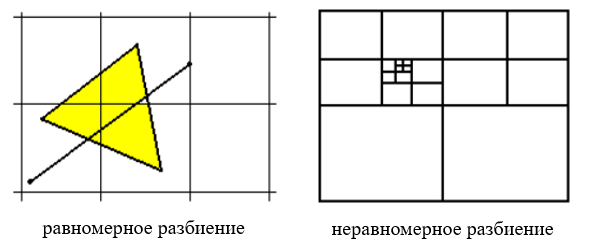
\includegraphics[width=\textwidth]{img/fig_partition.png}
    \caption{Равномерное и неравномерное разбиения пространства объектов}
    \label{fig:partition}
\end{figure}

	\item Иерархические древовидные структуры
	
При работе с большими объемами используются различные древовидные (иерархические) структуры. Стандартными формами таких структур являются восьмеричные (Octrees, для 3D), тетрарные (Quadtrees, для 2D), бинарные или BSP-деревья (Binary Space Partitioning Trees) и деревья ограничивающих тел. Иерархии позволяют упорядочивать грани объектов, производить быстрое и эффективное
отсечение граней, не удовлетворяющих каким-либо из условий.

\begin{enumerate}
	\item Иерархия ограничивающих тел
	
Получается дерево, корнем которого является тело, описанное вокруг всей сцены, а потомками – тела, описанные вокруг первичных, вторичных и др. групп.

Отсечение основного количества объектов происходит уже на ранней
стадии достаточно быстро, ценой всего лишь нескольких проверок.
	\item Иерархии разбиения
	
Каждая клетка исходного разбиения разбивается на части (которые, в свою очередь, так же могут быть разбиты и т.д. При этом каждая клетка разбиения соответствует узлу дерева).

Иерархии (как и разбиения) позволяют достаточно легко и просто
производить частичное упорядочение граней. В результате получается список граней, практически полностью упорядоченный,
что дает возможность применять специальные методы сортировки.
\end{enumerate}

\end{enumerate}

Специальные методы оптимизации:

\begin{enumerate}
	\item Потенциально видимые множества граней (препроцессинг построения PVS)
	\item Метод порталов (PVS "на ходу")
	\item Метод иерархических подсцен (модификация метода порталов)~\cite{tyrlapov}
\end{enumerate}

Ниже будут рассмотрены основные алгоритмы удаления  евидимых линий.



\subsubsection{Алгоритм плавающего горизонта}

\hspace{1.25cm}
Алгоритм плавающего горизонта чаще всего используется для удаления невидимых линий трёхмерного представления функций, описывающих поверхность в виде:

\[ F(x, y, z) = 0. \]

Подобные функции возникают во многих приложениях в математике, технике, естественных науках и других дисциплинах.

Предложено много алгоритмов, использующих этот подход. Поскольку в приложениях в основном интересуются описанием поверхности, этот алгоритм обычно работает в пространстве изображения. Главная идея данного метода заключается в сведении трехмерной задачи к двумерной путем пересечения исходной поверхности последовательностью параллельных секущих плоскостей, имеющих постоянные значения координат х, у или z.

\begin{figure}[H]
    \centering
    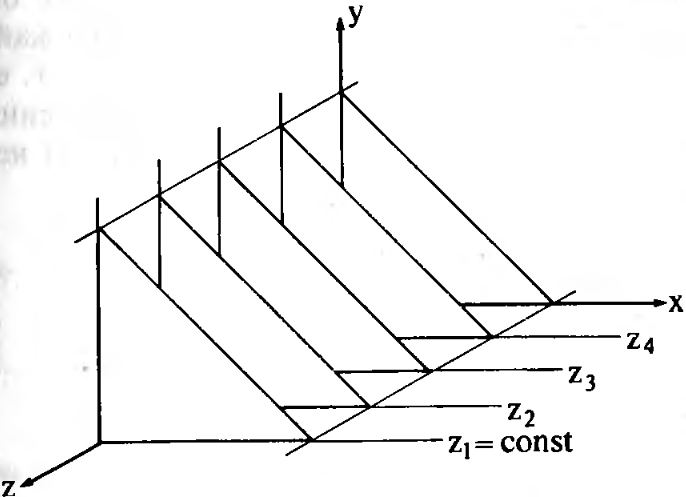
\includegraphics[width=0.7\textwidth]{img/floating_horizon_1.png}
    \caption{Секущие плоскости с постоянной координатой.}
    \label{fig:floating_horizon_1}
\end{figure}

\begin{figure}[H]
    \centering
    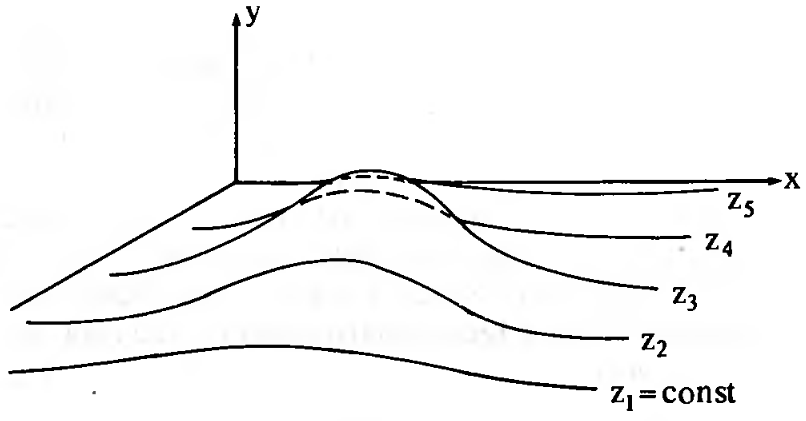
\includegraphics[width=0.7\textwidth]{img/floating_horizon_2.png}
    \caption{Кривые в секущих плоскостях с постоянной координатой.}
    \label{fig:floating_horizon_2}
\end{figure}

На рис.~\ref{fig:floating_horizon_1} приведен пример, где указанные параллельные плоскости определяются постоянными значениями \( z \). Функция \( F(x, y, z) = 0 \) сводится к последовательности кривых, лежащих в каждой из этих параллельных плоскостей, например, к последовательности

\[
y = f(x, z) \quad \text{или} \quad x = g(y, z)
\]

где \( z \) постоянно на каждой из заданных параллельных плоскостей.

Итак, поверхность теперь складывается из последовательности кривых, лежащих в каждой из этих плоскостей, как показано на рис.~\ref{fig:floating_horizon_2}. Здесь предполагается, что полученные кривые являются однозначными функциями независимых переменных. Если спроецировать полученные кривые на плоскость \( z = 0 \), как показано на рис.~\ref{fig:floating_horizon_3}, то сразу становится ясна идея алгоритма удаления невидимых участков исходной поверхности. Алгоритм сначала упорядочивает плоскости \( z = \text{const} \) по возрастанию расстояния до них от точки наблюдения. Затем для каждой плоскости, начиная с ближайшей к точке наблюдения, строится кривая, лежащая на ней, т.е. для каждого значения координаты \( x \) в пространстве изображения определяется соответствующее значение \( y \). Алгоритм удаления невидимой линии заключается в следующем:

\begin{figure}[H]
    \centering
    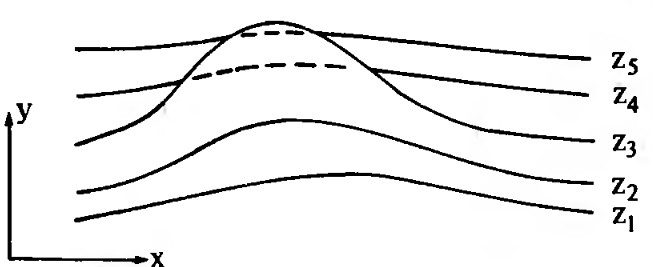
\includegraphics[width=0.7\textwidth]{img/floating_horizon_3.png}
    \caption{Проекция кривых на плоскость z = 0.}
    \label{fig:floating_horizon_3}
\end{figure}

Если на текущей плоскости при некотором заданном значении \( x \) соответствующее значение \( y \) на кривой больше значения \( y \) для всех предыдущих кривых при этом значении \( x \), то текущая кривая видима в этой точке; в противном случае она невидима.

Невидимые участки показаны пунктиром на рис.~\ref{fig:floating_horizon_3}. Реализация данного алгоритма достаточно проста. Для хранения максимальных значений \( y \) при каждом значении \( x \) используется массив, длина которого равна числу различимых точек (разрешению) по оси \( x \) в пространстве изображения. Значения, хранящиеся в этом массиве, представляют собой текущие значения «горизонта». Поэтому по мере рисования каждой очередной кривой этот горизонт «всплывает». Фактически этот алгоритм удаления невидимых линий работает каждый раз с одной линией. Алгоритм работает очень хорошо до тех пор, пока какая-нибудь очередная кривая не окажется ниже самой первой из кривых, как показано на рис.~\ref{fig:floating_horizon_4}~a.

\begin{figure}[H]
    \centering
    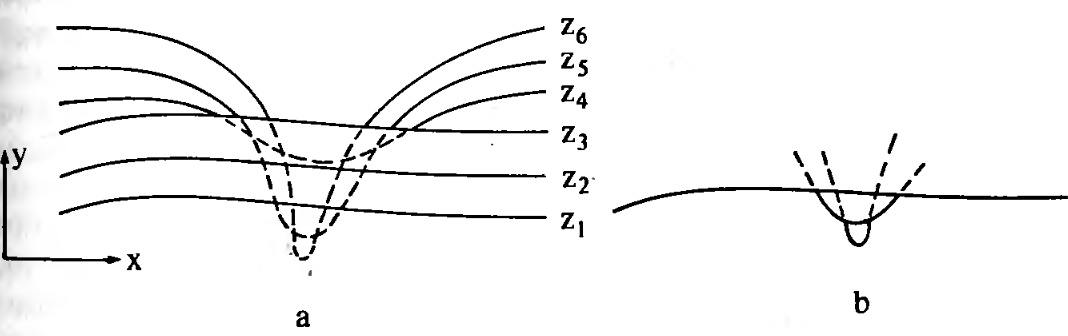
\includegraphics[width=\textwidth]{img/floating_horizon_4.png}
    \caption{Обработка нижней стороны поверхности.}
    \label{fig:floating_horizon_4}
\end{figure}

Подобные кривые, естественно, видимы и представляют собой нижнюю сторону исходной поверхности, однако алгоритм будет считать их невидимыми. Нижняя сторона поверхности делается видимой, если модифицировать этот алгоритм, включив в него нижний горизонт, который опускается вниз по ходу работы алгоритма. Это реализуется при помощи второго массива, длина которого равна числу различимых точек по оси \( x \) в пространстве изображения. Этот массив содержит наименьшие значения \( y \) для каждого значения \( x \). Алгоритм теперь становится таким:

Если на текущей плоскости при некотором заданном значении \( x \) соответствующее значение \( y \) на кривой больше максимума или меньше минимума по \( y \) для всех предыдущих кривых при этом \( x \), то текущая кривая видима. В противном случае она невидима.

Полученный результат показан на рис.~\ref{fig:floating_horizon_4}~b.

В изложенном алгоритме предполагается, что значение функции, т.е. \( y \), известно для каждого значения \( x \) в пространстве изображения. Однако если для каждого значения \( x \) нельзя указать (вычислить) соответствующее ему значение \( y \), то невозможно поддерживать массивы верхнего и нижнего плавающих горизонтов. В таком случае используется линейная интерполяция значений \( y \) между известными значениями для того, чтобы заполнить массивы верхнего и нижнего плавающих горизонтов, как показано на рис.~\ref{fig:floating_horizon_5}. Если видимость кривой меняется, то метод с такой простой интерполяцией не даст корректного результата. Этот эффект проиллюстрирован рис.~\ref{fig:floating_horizon_6}~a. Предполагая, что операция по заполнению массивов проводится после проверки видимости, получаем, что при переходе текущей кривой от видимого к невидимому состоянию (сегмент \( AB \) на рис.~\ref{fig:floating_horizon_6}~a), точка \( (X_{N+K}, Y_{N+K}) \) объявляется невидимой. Тогда участок кривой между точками \( (X_N, Y_N) \) и \( (X_{N+K}, Y_{N+K}) \) не изображается и операция по заполнению массивов не проводится. Образуется зазор между текущей и предыдущей кривыми. Если на участке текущей кривой происходит переход от невидимого состояния к видимому (сегмент \( CD \) на рис.~\ref{fig:floating_horizon_7}~a), то точка \( (X_{M+K}, Y_{M+K}) \) объявляется видимой, а участок кривой между точками \( (X_M, Y_M) \) и \( (X_{M+K}, Y_{M+K}) \) изображается и операция по заполнению массивов проводится. Поэтому изображается и невидимый кусок сегмента \( CD \). Кроме того, массивы плавающих горизонтов не будут содержать точных значений \( y \). А это может повлечь за собой дополнительные нежелательные эффекты для последующих кривых.

\begin{figure}[H]
    \centering
    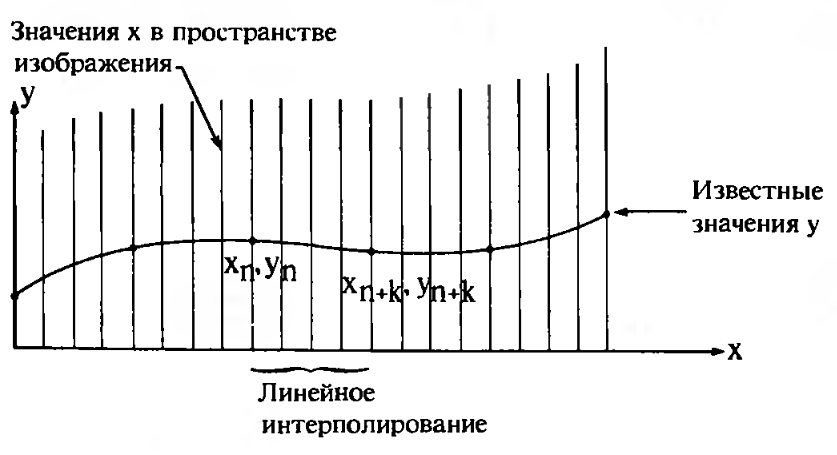
\includegraphics[width=0.8\textwidth]{img/floating_horizon_5.png}
    \caption{Линейная интерполяция между заданными точками.}
    \label{fig:floating_horizon_5}
\end{figure}

\begin{figure}[H]
    \centering
    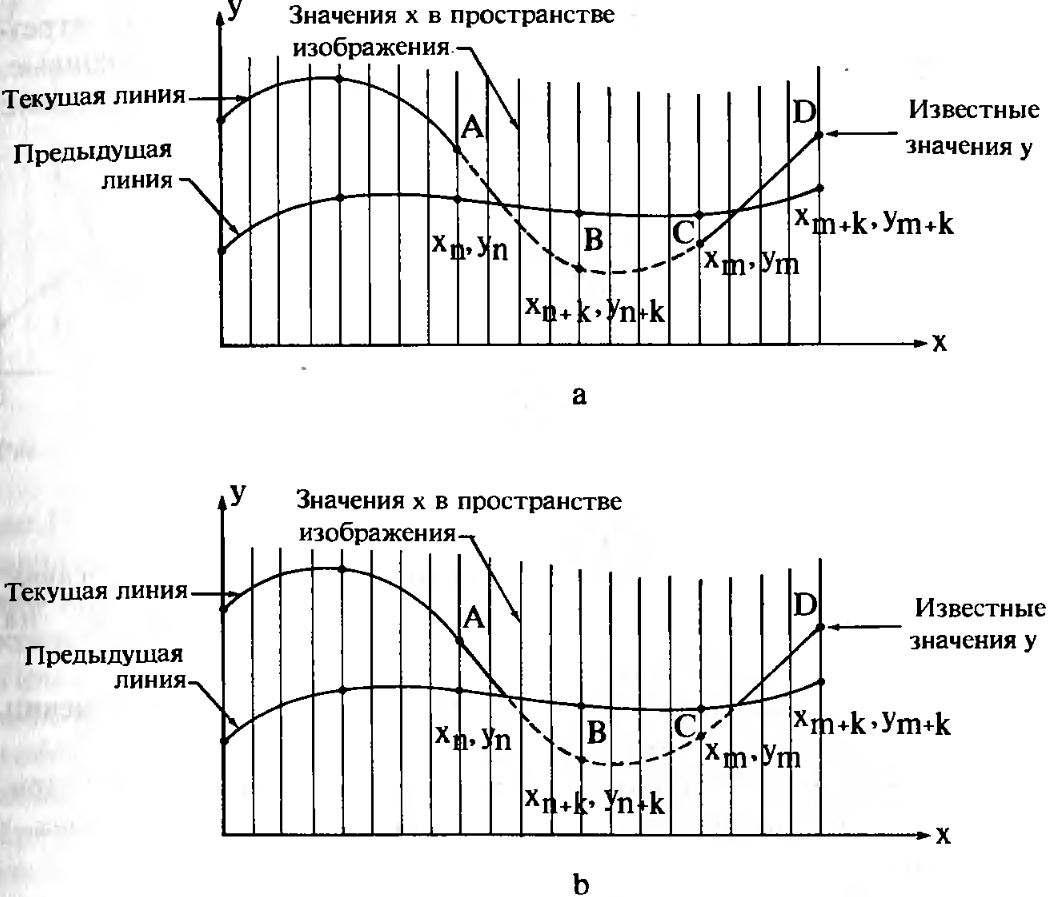
\includegraphics[width=0.8\textwidth]{img/floating_horizon_6.png}
    \caption{Эффект пересекающихся кривых.}
    \label{fig:floating_horizon_6}
\end{figure}

Следовательно, необходимо решать задачу о поиске точек пересечения сегментов текущей и предшествующей кривых.

Существует несколько методов получения точек пересечения кривых. На растровых дисплеях значение координаты \( x \) можно увеличивать на 1, начиная с \( x_n \) или \( x_m \) (рис.~\ref{fig:floating_horizon_6}~a). Значение \( y \), соответствующее текущему значению координаты \( x \) в пространстве изображения, получается путем добавления к значению \( y \), соответствующему предыдущему значению координаты \( x \), вертикального приращения \( \Delta y \) вдоль заданной кривой. Затем определяется видимость новой точки с координатами \( (x+1, y + \Delta y) \). Если эта точка видима, то активируется связанный с ней пиксел. Если невидима, то пиксел не активируется, а \( x \) увеличивается на 1. Этот процесс продолжается до тех пор, пока не встретится \( x_{n+k} \) или \( x_{m+k} \). Пересечения для растровых дисплеев определяются изложенным методом с достаточной точностью.

Теперь алгоритм излагается более формально.

Если на текущей плоскости при некотором заданном значении \( x \) соответствующее значение \( y \) на кривой больше максимума или меньше минимума по \( y \) для всех предыдущих кривых при этом \( x \), то текущая кривая видима. В противном случае она невидима. Если на участке от предыдущего \( x_n \) до текущего \( x_{n+k} \) значения \( x \) видимость кривой изменяется, то вычисляется точка пересечения \( x_i \). Если на участке от \( x_n \) до \( x_{n+k} \) сегмент кривой полностью видим, то он изображается целиком; если он стал невидимым, то изображается фрагмент от \( x_n \) до \( x_i \); если же он стал видимым, то изображается фрагмент от \( x_i \) до \( x_{n+k} \). Заполнить массивы верхнего и нижнего плавающих горизонтов.

Типичный результат работы алгоритма можно наблюдать на рисунке~\ref{fig:floating_horizon_7}.~\cite{rodgers}

\begin{figure}[H]
    \centering
    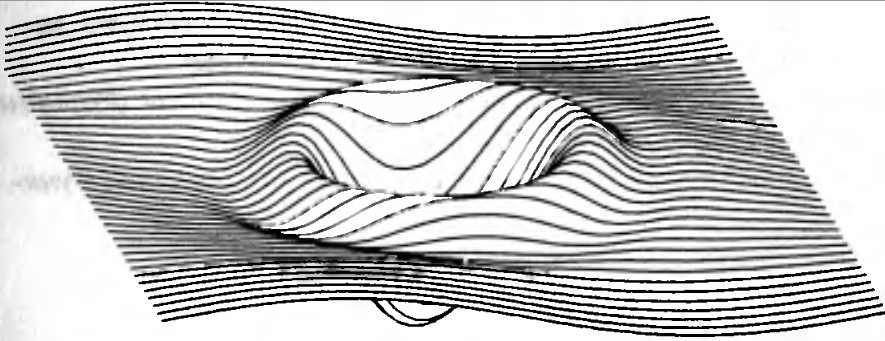
\includegraphics[width=\textwidth]{img/floating_horizon_7.png}
    \caption{Функция \( y = \frac{1}{5} \sin x \cos z - \frac{3}{2} \cos \left( \frac{7a}{4} \right) \times \exp(-a), \quad a = (x - \pi)^2 + (z - \pi)^2 \), изображенная в интервале \( (0, 2\pi) \) с помощью алгоритма плавающего горизонта.}
    \label{fig:floating_horizon_7}
\end{figure}



\subsubsection{Алгоритм Робертса}

\hspace{1.25cm}
Рассмотрим алгоритм удаления невидимых линий Робертса, требующий, чтобы каждая грань была выпуклым многоугольником.

Сначала отбрасываются все рёбра, обе определяющие грани которых являются нелицевыми (ни одно из таких рёбер заведомо не видно).

Следующим шагом является проверка на закрывание каждого из оставшихся рёбер со всеми лицевыми гранями многогранника. Возможны следующие случаи:

\begin{itemize}
    \item грань ребра не закрывает (рис.~\ref{fig:roberts_algorithm_1});

\begin{figure}[H]
    \centering
    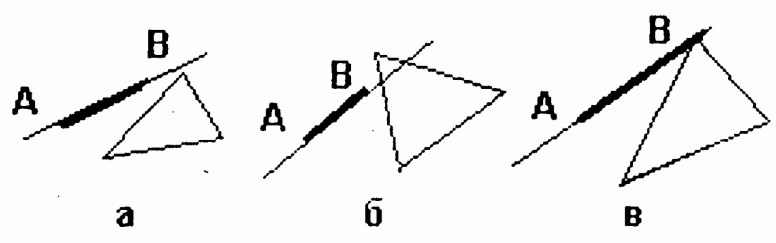
\includegraphics[width=\textwidth]{img/roberts_algorithm_1.png}
    \caption{Иллюстрация алгоритма Робертса: (а) грань не закрывает ребро, (б) грань частично закрывает ребро, (в) грань полностью закрывает ребро.}
    \label{fig:roberts_algorithm_1}
\end{figure}

	\item грань полностью закрывает ребро (тогда оно удаляется из списка рассматриваемых рёбер) (рис.~\ref{fig:roberts_algorithm_2}, а);
    \item грань частично закрывает ребро (в этом случае ребро разбивается на несколько частей, видимыми из которых являются не более двух; само ребро удаляется из списка, но в список проверяемых рёбер добавляются те его части, которые данной гранью не закрываются).
\end{itemize}

Рассмотрим, как осуществляются эти проверки.

Пусть задано ребро \( AB \), где точка \( A \) имеет координаты \( (x_a, y_a) \), а точка \( B \) --- \( (x_b, y_b) \).

Прямая, проходящая через отрезок \( AB \), задаётся уравнениями
\[
x = x_a + t (x_b - x_a), \quad y = y_a + t (y_b - y_a)
\]
причем сам отрезок соответствует значениям параметра \( 0 \leq t \leq 1 \).

Данную прямую можно задать неявным образом как \( F(x, y) = 0 \), где
\[
F(x, y) = (y_b - y_a)(x - x_a) - (y - y_a)(x_b - x_a).
\]

Предположим, что проекция грани задается набором проекций вершин \( P_1, \dots, P_k \) с координатами \( (x_i, y_i) \), \( i = 1, \dots, n \). Обозначим через \( F_i \) значение функции \( F \) в точке \( P_i \).

Рассмотрим \( i \)-й отрезок проекции грани \( P_i P_{i+1} \). Этот отрезок пересекает прямую \( AB \) тогда и только тогда, когда функция \( F \) принимает значения разных знаков на концах этого отрезка, а именно при
\[
F_i F_{i+1} \leq 0.
\]

Случай, когда \( F_i F_{i+1} = 0 \), будем отбрасывать, чтобы дважды не засчитывать прямую, проходящую через вершину, для обоих выходящих из неё отрезков.

Итак, мы считаем, что пересечение имеет место в двух случаях:
\[
F_i \geq 0, \; F_{i+1} < 0,
\]
\[
F_i \leq 0, \; F_{i+1} > 0.
\]

Точка пересечения определяется соотношениями
\[
x = x_i + s(x_{i+1} - x_i),
\]
\[
y = y_i + s(y_{i+1} - y_i),
\]
где \( s = \frac{F_i}{F_i - F_{i+1}} \).

Отсюда легко находится значение параметра \( t \):
\[
t = 
\begin{cases} 
    \frac{x - x_a}{x_b - x_a}, & |x_b - x_a| \geq |y_b - y_a|, \\ 
    \frac{y - y_a}{y_b - y_a}, & |y_b - y_a| > |x_b - x_a|. 
\end{cases}
\]

Возможны следующие случаи:

\begin{enumerate}

    \item Отрезок не имеет пересечений с проекцией грани, кроме, быть может, одной точки. Это может иметь место, когда
\begin{itemize}

	\item прямая \( AB \) не пересекает рёбра проекции грани (рис.~\ref{fig:roberts_algorithm_1}, а);

    \item прямая \( AB \) пересекает ребра в двух точках \( t_1 \) и \( t_2 \), но либо \( t_1 < 0 \), \( t_2 < 0 \), либо \( t_1 > 1 \), \( t_2 > 1 \) (рис.~\ref{fig:roberts_algorithm_1}, б);
    \item прямая \( AB \) проходит через одну вершину, не задевая внутренности треугольника (рис.~\ref{fig:roberts_algorithm_1}, в).
\end{itemize}

Очевидно, что в этом случае соответствующая грань никак не может закрывать собой ребро \( AB \).

    \item Проекция ребра полностью содержится внутри проекции грани (рис.~\ref{fig:roberts_algorithm_2}, а). Тогда есть две точки пересечения прямой \( AB \) и границы грани и \( t_1 < 0 < t_2 < 1 \). Если грань лежит ближе к картинной плоскости, чем ребро, то ребро полностью невидимо и удаляется.
    
    \item Прямая \( AB \) пересекает ребра проекции грани в двух точках и либо \( t_1 < 0 \leq t_2 \leq 1 \), либо \( 0 < t_1 \leq 1 < t_2 \) (рис.~\ref{fig:roberts_algorithm_2}, б и в). Если ребро \( AB \) находится дальше от картинной плоскости, чем соответствующая грань, то оно разбивается на две части, одна из которых полностью закрывается гранью и потому отбрасывается. Проекция второй части лежит вне проекции грани и поэтому этой гранью не закрывается.
    
\begin{figure}[H]
    \centering
    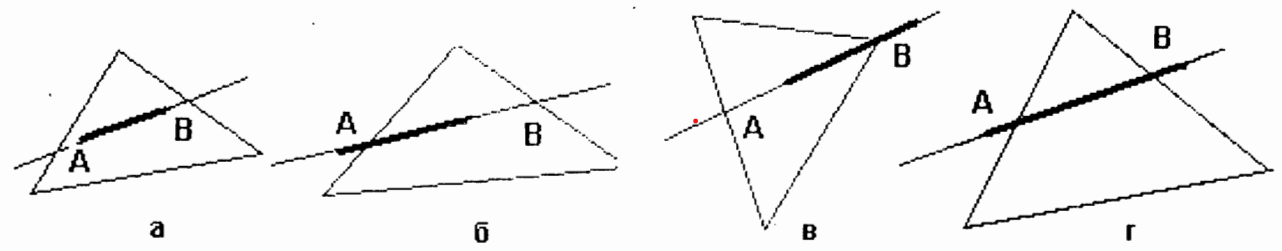
\includegraphics[width=\textwidth]{img/roberts_algorithm_2.png}
    \caption{}
    \label{fig:roberts_algorithm_2}
\end{figure}    
    
    \item Прямая \( AB \) пересекает ребра проекции грани в двух точках, причем \( 0 < t_1 < t_2 < 1 \) (рис.~\ref{fig:roberts_algorithm_2}, г). Если ребро \( AB \) лежит дальше от картинной плоскости, чем соответствующая грань, то оно разбивается на три части, средняя из которых отбрасывается.

\end{enumerate}

Для определения того, что лежит ближе к картинной плоскости — отрезок \( AB \) (проекция которого лежит в проекции грани) или сама грань, через эту грань проводится плоскость
\[
(n, p) + c = 0
\]
(\( n \) — нормальный вектор грани), разбивающая всё пространство на два полупространства. Если оба конца отрезка \( AB \) лежат в том же полупространстве, в котором находится и наблюдатель, то отрезок лежит ближе к грани; если оба конца находятся в другом полупространстве, то отрезок лежит дальше. Случай, когда концы лежат в разных полупространствах, здесь невозможен (это означало бы, что отрезок \( AB \) пересекает внутреннюю часть грани).

Если общее количество граней равно \( n \), то временные затраты для данного алгоритма составляют \( O(n^2) \).

Количество проверок можно заметно сократить, если воспользоваться разбиением картинной плоскости.

Разобьем видимую часть картинной плоскости (экран) на \( N_1 \times N_2 \) равных частей (клеток) и для каждой клетки \( A_{ij} \) построим список всех лицевых граней, чьи проекции имеют с данной клеткой непустое пересечение.

Для проверки произвольного ребра на пересечение с гранями отберем сначала все те клетки, которые проекция данного ребра пересекает. Ясно, что проверять на пересечение с ребром имеет смысл только те грани, которые содержатся в списках этих клеток.

В качестве шага разбиения обычно выбирается \( O(l) \), где \( l \) — характерный размер ребра в сцене. Для любого ребра количество проверяемых граней практически не зависит от общего числа граней и совокупные временные затраты алгоритма на проверку пересечений составляют \( O(n) \), где \( n \) — количество ребер в сцене.

Поскольку процесс построения списков заключается в переборе всех граней, их проектировании и определении клеток, в которые попадают проекции, то затраты на составление всех списков также составляют \( O(n) \).~\cite{shishkin}




\subsubsection{Алгоритм Варнака}

\hspace{1.25cm}
Джон Варнак, американский учёный, один из основателей компании
Adobe Systems. Алгоритм Варнака позволяет определить, какие грани или части граней объектов сцены видимы, а какие заслонены гранями
других объектов. Так же как и в алгоритме Робертса анализ видимости
происходит в картинной плоскости. В качестве граней обычно выступают
выпуклые многоугольники, алгоритмы работы с ними эффективнее, чем с
произвольными многоугольниками. Окно, в котором необходимо отобразить сцену, должно быть прямоугольным. Алгоритм работает рекурсивно, на каждом шаге анализируется видимость граней и, если нельзя легко определить видимость, окно делится на 4 части и анализ повторяется отдельно для каждой из частей (см. рис.~\ref{fig:varnak_algorithm_1}).

Случаи, когда можно легко определить видимость, следующие:

\begin{enumerate}
	\item в окне нет ни одной грани, в этом случае ничего рисовать не нужно;
	\item в окне ровно одна грань, в этом случае достаточно отобразить эту
грань, так как нет других граней, которые могли бы её заслонить;
	\item размеры окна равны размерам одного пиксела, в этом случае из
граней выбирается ближайшая и её цветом закрашивается этот
пиксел;
	\item ближайшая грань охватывает всё окно, в этом случае она заслоняет все остальные грани и достаточно отобразить только её. 
\end{enumerate}

\begin{figure}[H]
    \centering
    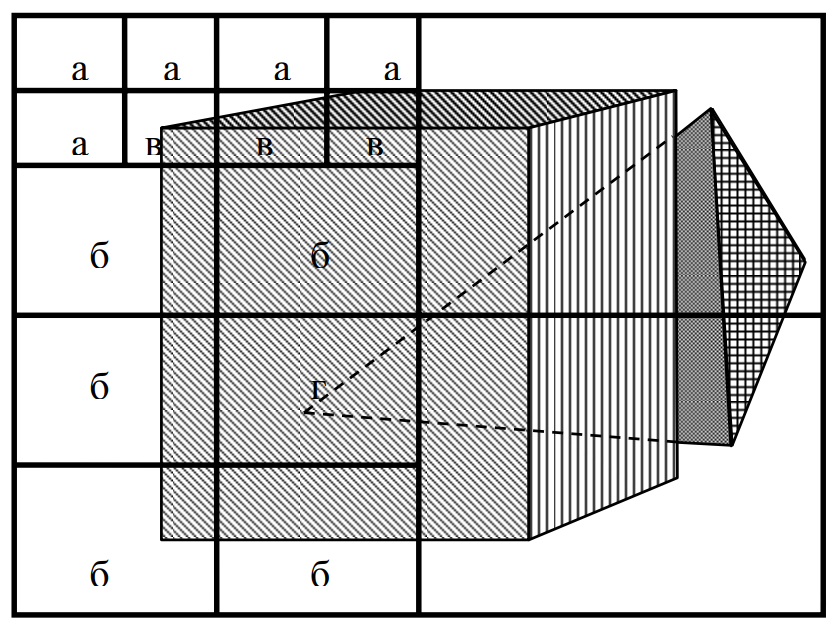
\includegraphics[width=0.9\textwidth]{img/varnak_algorithm_1.png}
    \caption{Определение видимости алгоритмом Варнака.}
    \label{fig:varnak_algorithm_1}
\end{figure}

Алгоритм можно разделить на следующие элементарные задачи:

\begin{itemize}
	\item определение, в какие части окна попадает грань;
	\item определение, что грань охватывает окно;
	\item определение, что грань является ближайшей.
\end{itemize}

Существует два различных подхода к решению этих задач. Сначала
рассмотрим вариант решения первой задачи, когда при разделении окна
грани разрезаются на части вертикальной и горизонтальной прямыми, делящими окно. Получившиеся многоугольники полностью лежат в соответствующих частях окна, и заносятся в соответствующий этой части набор.
При последующем делении окна они разрезаются на более мелкие части.
Определить, что такой многоугольник охватывает всё окно можно по условию, что каждая из четырёх вершин окна совпадает с одной из вершин
многоугольника. Определить, что грань ближайшая можно по глубине
вершин многоугольника. При перспективной проекции в качестве параметра глубины удобно использовать обратную величину \(w = 1/z\), где z – координата глубины, так как w в отличие от z можно линейно интерполировать в экранных координатах. Чем больше w, тем ближе вершина к наблюдателю. Так как грань не обязательно параллельна экрану, то глубина у
вершин разная. Найдя минимум и максимум глубины всех вершин можно
определить интервал глубины [Wmin, Wmax]. В случае, когда окно равно
пикселу, достаточно выбрать грань с максимальным Wmax, она и будет
ближайшей. Если же нужно убедиться, что грань ближе всех остальных
граней, то необходимо проверить условие, что Wmin этой грани больше
Wmax всех остальных граней.

Второй подход не требует деления граней на части, для вычислений
всегда используются исходные грани.

Для решения первой задачи нужно определить факт пересечения
двух выпуклых многоугольников – грани и окна. Это можно сделать, например, по следующему условию: многоугольники не пересекаются, если
все вершины одного из них лежат с внешней стороны от прямой, образующей ребро другого (см. рис.~\ref{fig:varnak_algorithm_2}). Нужно перебрать все рёбра грани и сравнить с вершинами окна, и все четыре границы окна сравнить с вершинами грани.

\begin{figure}[H]
    \centering
    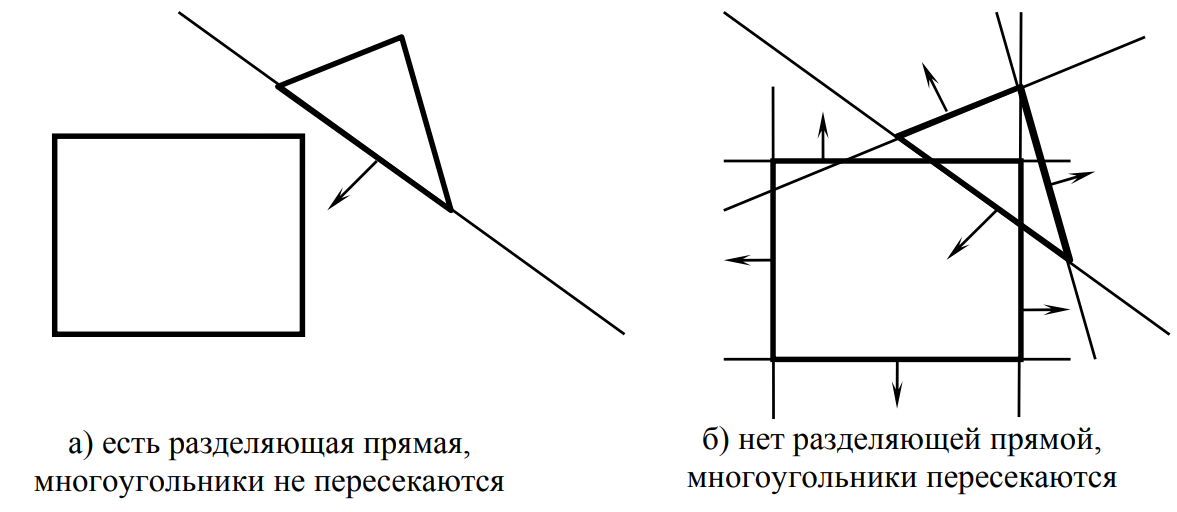
\includegraphics[width=\textwidth]{img/varnak_algorithm_2.png}
    \caption{Определение пересечения выпуклых многоугольников.}
    \label{fig:varnak_algorithm_2}
\end{figure}

Для решения второй задачи достаточно проверить, что все 4 угла окна лежат внутри или на границе грани. Это можно определить по расстояниям от углов окна до прямых, образующих рёбра граней.

Третья задача решается сложнее, чем в первом варианте. Грань не
лежит полностью в окне, поэтому рассчитывать интервал её глубины по
вершинам будет неправильно. Необходимы вершины той её части, которая
лежит в окне. Это вершины грани, попадающие в окно, вершины окна, попадающие в грань и точки пересечения рёбер грани с рёбрами окна (см.
рис.~\ref{fig:varnak_algorithm_3}).

По этим точкам рассчитывается интервал глубины [Wmin, Wmax] и
используется для определения ближайшей грани.

\begin{figure}[H]
    \centering
    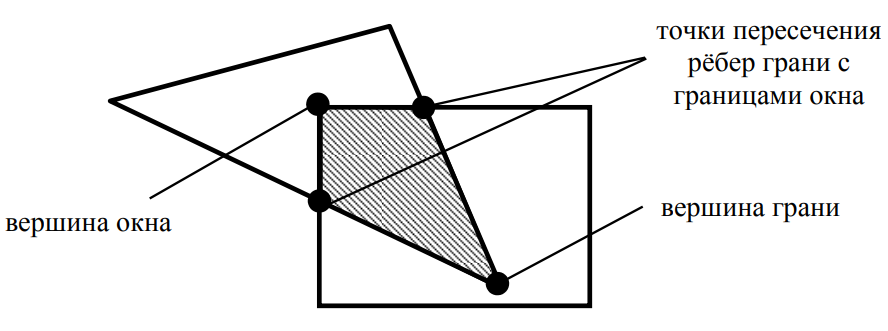
\includegraphics[width=\textwidth]{img/varnak_algorithm_3.png}
    \caption{Определение вершин пересечения грани с окном.}
    \label{fig:varnak_algorithm_3}
\end{figure}

У каждого из подходов есть свои достоинства и недостатки. Подход
с разрезанием граней проще в реализации, но требует дополнительной памяти для хранения частей граней. Второй подход лишён этого недостатка,
но более сложен в реализации. Производительность при обоих подходах
примерно одинакова. Её можно оценить, исходя из количества граней N и
количества пикселей C как O(CN), так как в худшем случае все грани могут быть размером с окно и окно в худшем случае придётся делить до пиксела. Уменьшить количество граней нельзя, но можно сократить количество делений окна. Например, его можно сократить, если дополнительно обрабатывать случай на общем ребре двух граней. По описанному алгоритму окно, в которое попадает общее ребро двух граней, будет делиться до пиксела. Это происходит потому, что не выполняется ни один из четырёх случаев, в окне несколько граней и ни одна из этих граней не охватывает окно (см. рис.~\ref{fig:varnak_algorithm_4}).

\begin{figure}[H]
    \centering
    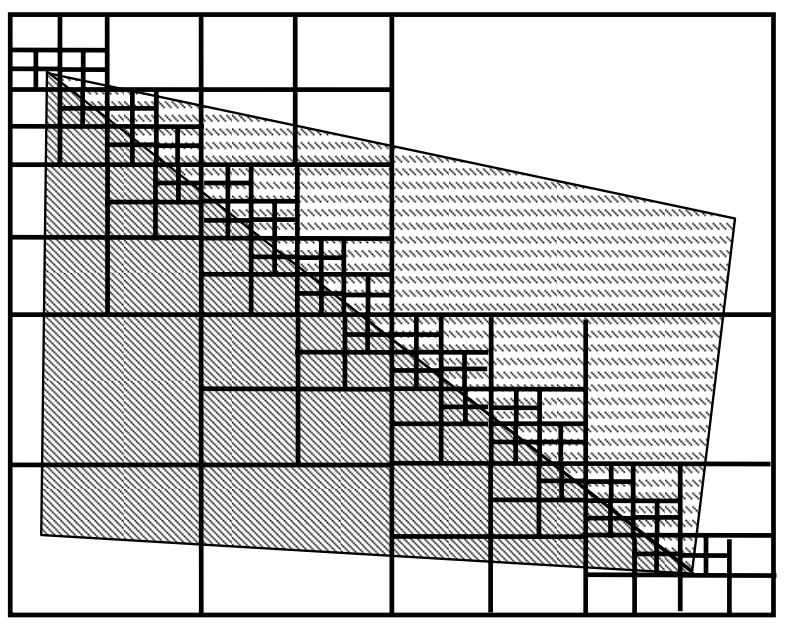
\includegraphics[width=\textwidth]{img/varnak_algorithm_4.png}
    \caption{Разделение окна вдоль общего ребра двух граней.}
    \label{fig:varnak_algorithm_4}
\end{figure}

Можно избежать лишних делений, если выделить общие рёбра граней, и добавить ещё один простой случай: две грани с общим ребром полностью охватывают окно и являются ближайшими. Ребро в этом случае
должно пересекать окно в двух точках, вершины окна с одной стороны
ребра должны лежать внутри грани лежащей с этой стороны ребра, а вершины окна с другой стороны ребра должны лежать внутри второй грани
(см. рис.~\ref{fig:varnak_algorithm_5}).

\begin{figure}[H]
    \centering
    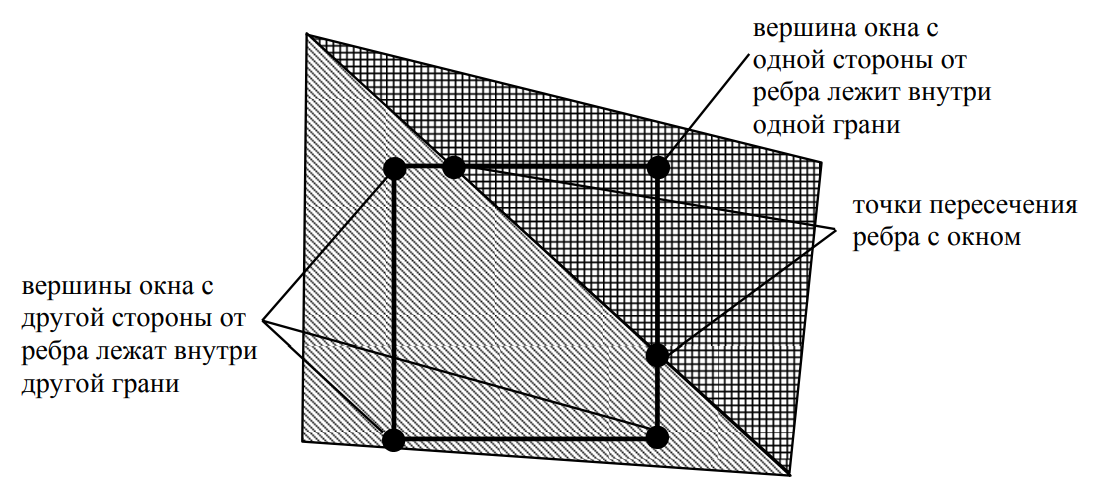
\includegraphics[width=\textwidth]{img/varnak_algorithm_5.png}
    \caption{Определение случая с двумя гранями с общим ребром.}
    \label{fig:varnak_algorithm_5}
\end{figure}

Интервал глубины [Wmin, Wmax] должен рассчитываться по вершинам обеих граней, попавших в окно частей.~\cite{polski}




\subsubsection{Алгоритм Вейлера-Азертона}

\hspace{1.25cm}
Вейлер и Азертон попытались минимизировать количество шагов в алгоритме разбиения типа алгоритма Варнока путем разбиения окна вдоль границ многоугольника. Выходными данными этого алгоритма, который для достижения необходимой точности работает в пространстве объекта, служат многоугольники. Поскольку выходом являются многоугольники, то алгоритм можно легко использовать для удаления как невидимых линий, так и невидимых поверхностей. Алгоритм удаления невидимых поверхностей состоит из четырех шагов.

\begin{enumerate}
    \item Предварительная сортировка по глубине.
    \item Отсечение по границе ближайшего к наблюдателю многоугольника, называемое сортировкой многоугольников на плоскости.
    \item Удаление многоугольников, экранированных многоугольником, ближайшим к точке наблюдения.
    \item Если требуется, то рекурсивное подразделение и окончательная сортировка для устранения всех неопределенностей.
\end{enumerate}

Предварительная сортировка по глубине нужна для формирования списка приблизительных приоритетов. Предположим, что точка наблюдения расположена в бесконечности на положительной полуоси \(z\), тогда ближайшим к ней и первым в списке будет тот многоугольник, который обладает вершиной с максимальной координатой \(z\).

\begin{figure}[H]
    \centering
    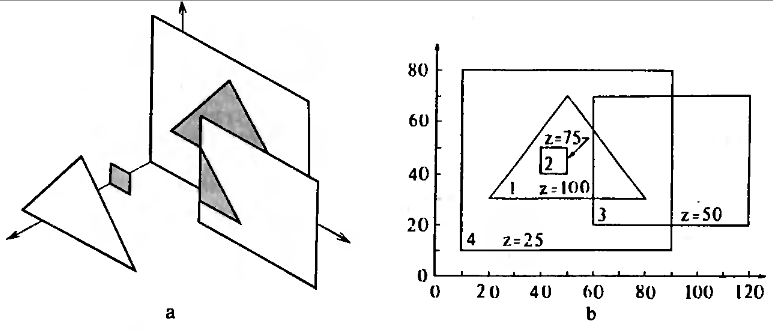
\includegraphics[width=\textwidth]{img/veyler-aserton_algorithm_1.png}
    \caption{Отсечение многоугольников по приоритетам для алгоритма удаления невидимых поверхностей Вейлера — Азертона.}
    \label{fig:veyler-aserton_algorithm_1}
\end{figure}

В качестве отсекающего многоугольника используется копия первого многоугольника из предварительного списка приоритетов по глубине. Отсекаться будут оставшиеся в этом списке многоугольники, включая и первый многоугольник. Вводятся два списка: внутренний и внешний. С помощью алгоритма отсечения Вейлера — Азертона все многоугольники отсекаются по границам отсекающего многоугольника. Фактически это двумерная операция отсечения проекций отсекающего и отсекаемого многоугольников. Та часть каждого отсекаемого многоугольника, которая оказывается внутри отсекающего, если она имеется, попадает во внутренний список. Оставшаяся часть, если таковая есть, попадает во внешний список. Этот этап алгоритма является сортировкой на плоскости или \(xy\)-сортировкой. Пример приведен на рис.~\ref{fig:veyler-aserton_algorithm_1}. На рис.~\ref{fig:veyler-aserton_algorithm_2} показаны внутренний и внешний списки для сцены на рис.~\ref{fig:veyler-aserton_algorithm_1}. Теперь сравниваются глубины каждого многоугольника из внутреннего списка с глубиной отсекающего многоугольника. С использованием координат \((x, y)\) вершин отсекаемых многоугольников и уравнений несущих плоскостей вычисляются глубины (координаты \(z\)) каждой вершины. Затем они сравниваются с минимальной координатой \(z(z_{\text{min}})\) для отсекающего многоугольника. Если глубина ни одной из этих вершин не будет больше \(z_{\text{min}}\), то все многоугольники из внутреннего списка экранируются отсекающим многоугольником (рис.~\ref{fig:veyler-aserton_algorithm_1}). Эти многоугольники удаляются, и выбирается следующий многоугольник. Заметим, что во внутренний список остается лишь отсекающий многоугольник. Работа алгоритма затем продолжается с внешним списком.

\begin{figure}[H]
    \centering
    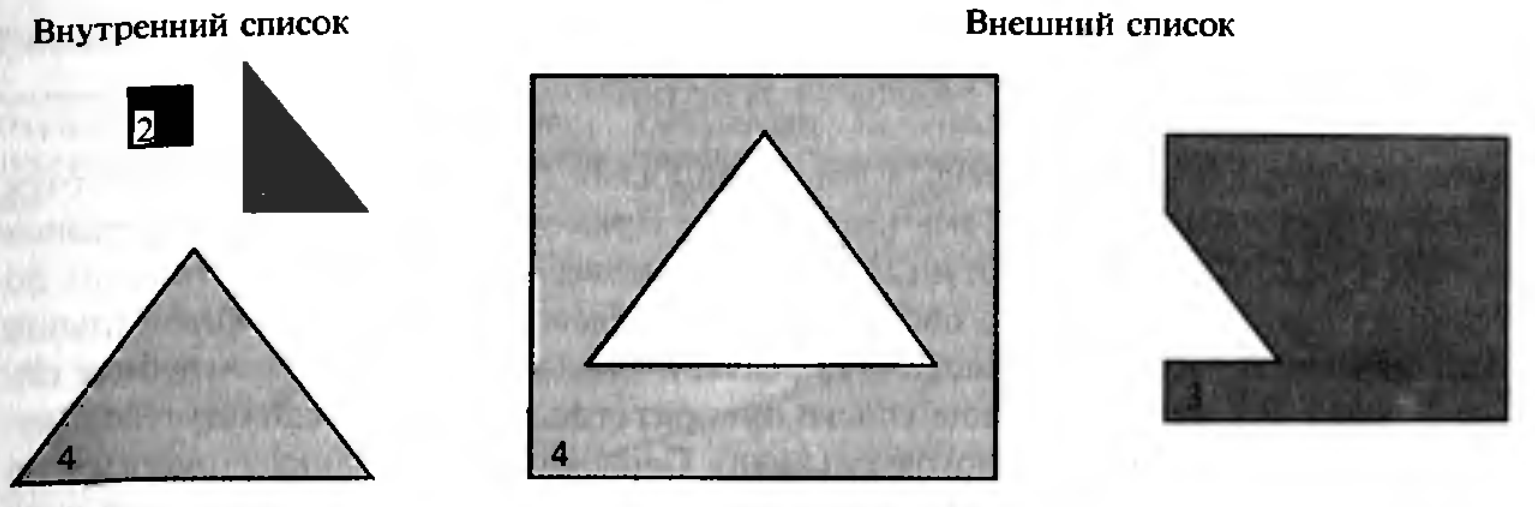
\includegraphics[width=\textwidth]{img/veyler-aserton_algorithm_2.png}
    \caption{Внутренний и внешний списки многоугольников.}
    \label{fig:veyler-aserton_algorithm_2}
\end{figure}

Если координата \(z\) какого-либо многоугольника из внутреннего списка окажется больше, чем \( z_{\text{c min}} \), то такой многоугольник по крайней мере частично экранирует отсекающий многоугольник. На рис.~\ref{fig:veyler-aserton_algorithm_3} показано, как это может произойти. В подобном случае результат предварительной сортировки по глубине ошибочен. Поэтому алгоритм рекурсивно подразделяет плоскость \( (x, y) \), используя многоугольник, нарушивший порядок, в качестве нового отсекающего многоугольника. Отсечению подлежат многоугольники из внутреннего списка, причем старый отсекающий многоугольник теперь сам будет подвергнут отсечению новым отсекающим многоугольником. Подчеркнем, что новый отсекающий многоугольник является копией исходного многоугольника, а не его остатка после первого отсечения. Использование копии неотсекаемого многоугольника позволяет минимизировать число разбиений.

\begin{figure}[H]
    \centering
    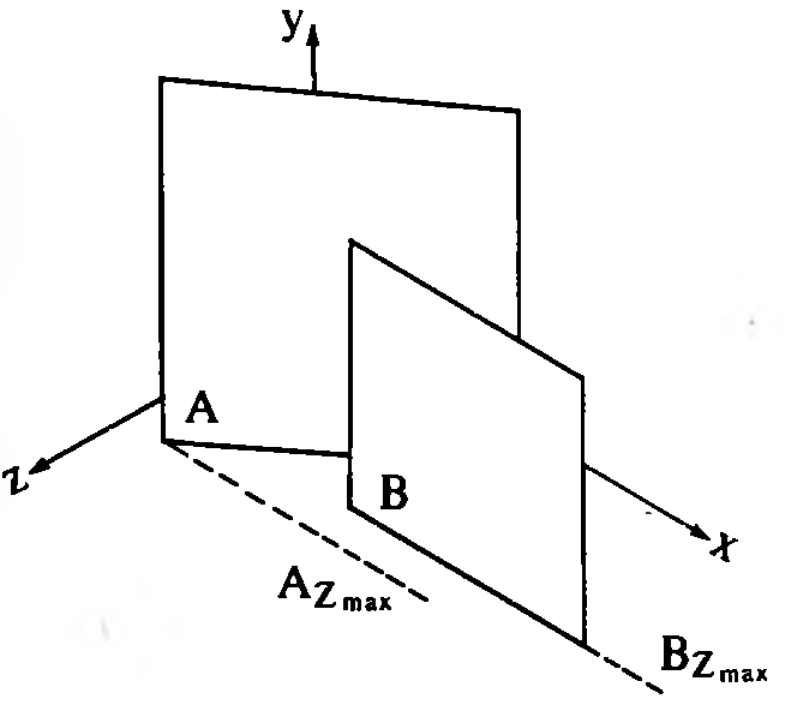
\includegraphics[width=0.6\textwidth]{img/veyler-aserton_algorithm_3.png}
    \caption{Условие возникновения
ошибочного результата в предвари-
тельной сортировке по z.}
    \label{fig:veyler-aserton_algorithm_3}
\end{figure}

Заслуживает внимание еще одна дополнительная деталь этого алгоритма. Когда некоторый многоугольник циклически перекрывается с отсекающим, т. е. когда он лежит как впереди, так и позади отсекающего (рис.~\ref{fig:veyler-aserton_algorithm_4}, а), то в рекурсоном разбиении необходимости нет. дело в том, что все экранируемое циклическим многоугольником уже было удалено на предыдущем шаге отсечения. Необходимо лишь произвести отсечение исходного многоугольника по границам циклического многоугольника и изобразить результат. Ненужное рекурсивное разбиение можно предотвратить, если создать список многоугольников, которые уже использовались как отсекающие. Тогда, если при рекурсивном разбиении текущий отсекающий многоугольник появляется в этом списке, значит, обнаружен циклически перекрывающийся многоугольник. Следовательно, не требуется никакого дополнительного разбиения. Заметим, что данный алгоритм непосредственно обрабатывает случаи циклического перекрытия сразу нескольких многоугольников, как показано на рис.~\ref{fig:veyler-aserton_algorithm_4}, b.~\cite{rodgers}

\begin{figure}[H]
    \centering
    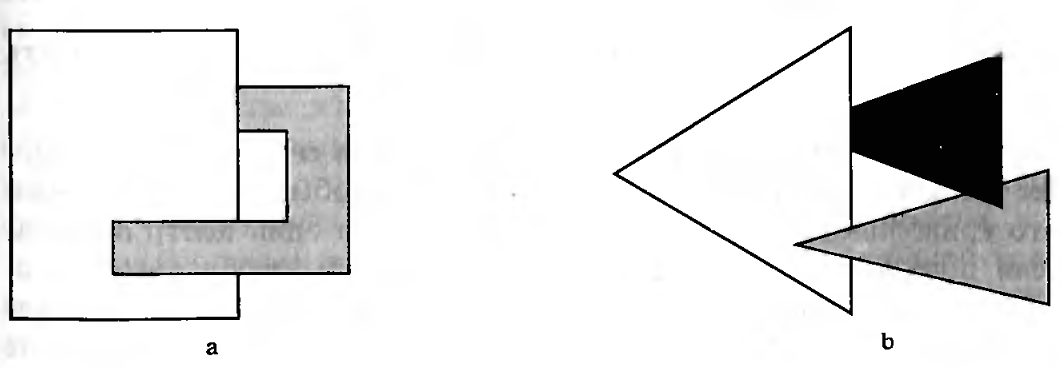
\includegraphics[width=\textwidth]{img/veyler-aserton_algorithm_4.png}
    \caption{Циклически перекрывающиеся многоугольники.}
    \label{fig:veyler-aserton_algorithm_4}
\end{figure}


\subsubsection{Алгоритм художника}

\hspace{1.25cm}
Алгоритм художника позволяет определить, какие пикселы граней сцены видимы, а какие заслонены гранями других объектов. Для этого все грани сортируются и рисуются в порядке от дальних к ближним, в результате чего ближние грани автоматически заслоняют дальние (см. рис.~\ref{fig:artist_algorithm_1}).

\begin{figure}[H]
    \centering
    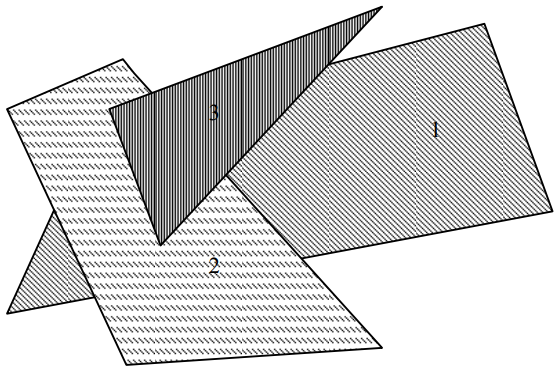
\includegraphics[width=0.7\textwidth]{img/artist_algorithm_1.png}
    \caption{Отрисовка граней по алгоритму художника.}
    \label{fig:artist_algorithm_1}
\end{figure}

Сортировка граней от дальних к ближним задача нетривиальная, недостаточно отсортировать грани по координате, соответствующей глубине. Каждой грани обычно соответствует некоторый интервал глубины, и если интервалы двух граней пересекаются, то нужны дополнительные проверки, чтобы определить, какая грань ближе. Кроме того, встречаются ситуации, когда грани отсортировать невозможно, например, когда грани образуют цикл (см. рис.~\ref{fig:artist_algorithm_2}а). В этом случае нужно разделить одну из граней на части (см. рис.~\ref{fig:artist_algorithm_2}б), и тогда становится возможным определить порядок рисования.

\begin{figure}[H]
    \centering
    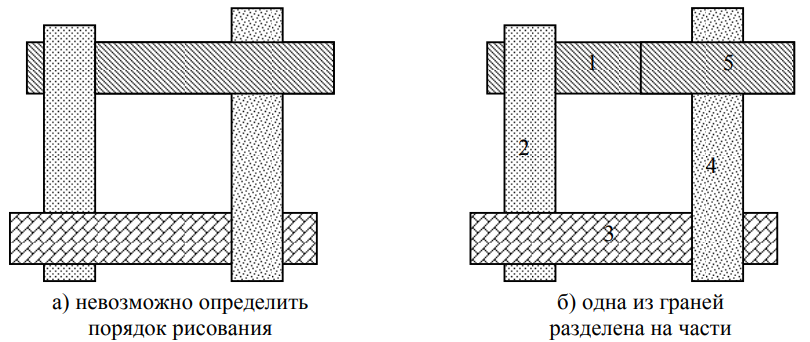
\includegraphics[width=\textwidth]{img/artist_algorithm_2.png}
    \caption{Циклически закрывающие друг друга грани.}
    \label{fig:artist_algorithm_2}
\end{figure}

Одним из методов сортировки граней является метод бинарного разделения пространства. В качестве исходных данных выступает набор граней в пространстве и точка, в которой находится наблюдатель. Если разделить пространство плоскостью одной из граней, то грани, лежащие в полупространстве, в котором находится наблюдатель, будут ближе к нему, чем те, что лежат в другом полупространстве. Поэтому порядок рисования граней будет следующим:

\begin{enumerate}
\item грани, лежащие в полупространстве, где нет наблюдателя;
\item грани, лежащие на разделяющей плоскости;
\item грани, лежащие в полупространстве, где находится наблюдатель.
\end{enumerate}

Аналогично сортируются и грани в полупространствах, в каждом выбирается грань, её плоскостью полупространство делится на две части и так до тех пор, пока в каждой части не останется ни одной грани.
В качестве примера рассмотрим случай на плоскости (см. рис.~\ref{fig:artist_algorithm_3}),
вместо граней – отрезки (a, b, c, d, e, f, g, h), вместо плоскостей – прямые (можно представить, что все грани вертикальные, а на рисунке показан их вид сверху).

\begin{figure}[H]
    \centering
    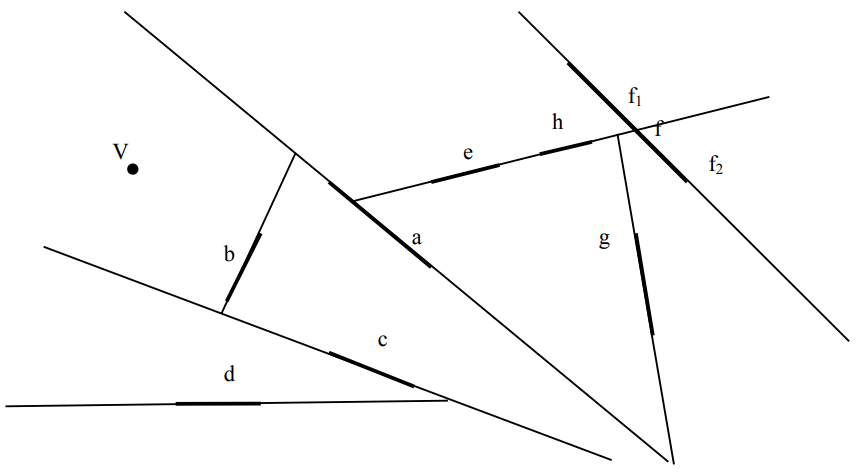
\includegraphics[width=\textwidth]{img/artist_algorithm_3.png}
    \caption{Сортировка граней бинарным разделением пространства.}
    \label{fig:artist_algorithm_3}
\end{figure}

Наблюдатель находится в точке $V$. Плоскость первой грани ($a$) делит грани на три группы: 
\begin{itemize}
    \item ($b, c, d$) – лежат в полупространстве наблюдателя,
    \item ($e, g, h, f$) – в другом полупространстве,
    \item грань ($a$) – на разделяющей плоскости.
\end{itemize}
Порядок рисования: ($e, g, h, f$), ($a$), ($b, c, d$). Грани в каждом из полупространств нужно отсортировать между собой. 
В одном выбирается плоскость грани ($e$), она делит грани на группы:
\begin{itemize}
    \item ($f_1$) – лежит в полупространстве наблюдателя,
    \item ($f_2, g$) – в другом полупространстве,
    \item грани ($e, h$) – на разделяющей плоскости.
\end{itemize}
Грань ($f$) попала в оба полупространства и была разделена на две части ($f_1$ и $f_2$), грань ($h$) попала на разделяющую плоскость и должна рисоваться вместе с гранью ($e$). Их взаимный порядок рисования может быть любым, так как они не могут заслонить друг друга, находясь в одной плоскости. 

Аналогично, в части пространства с гранями ($f_2, g$) выбирается плоскость $g$, а в части пространства с гранями ($b, c, d$) – грань ($c$). После всех разделений порядок рисования граней будет: 
\[
f_2, g, e, h, f_1, a, d, c, b.
\]

Время, необходимое на сортировку, зависит от количества граней на всех этапах разделения пространства. Например, при первом делении нужно сравнить с разделяющей плоскостью все $N$ граней. Количество граней может возрасти из-за разделения граней на части, поэтому лучше выбирать такие плоскости, которые делят минимум граней. Также алгоритм будет работать эффективнее, если с каждой стороны от разделяющей плоскости будет примерно одинаковое количество граней.

Рассмотрим два крайних случая:
\begin{enumerate}
    \item Все грани оказываются с одной стороны от плоскости, кроме одной, которая является разделяющей. Тогда количество сравнений на первом шаге будет $N$, на втором $N-1$, на третьем $N-2$ и так далее до $1$. Общее количество делений будет $N$, а сложность $O(N^2)$.
    \item Грани с обеих сторон распределены поровну. Количество сравнений на первом шаге будет $N$, на втором $N/2 + N/2$ (по $N/2$ с каждой стороны), на третьем $N/4 + N/4 + N/4 + N/4$ и так далее, пока не останется $1 + 1 + \ldots + 1$. Общее количество делений будет $\log N$, а сложность $O(N \cdot \log N)$.~\cite{polski}
\end{enumerate} 


\subsubsection{Алгоритм трассировки лучей}

\hspace{1.25cm}
Алгоритм трассировки лучей позволяет определить, какие пикселы граней сцены видимы, а какие заслонены гранями других объектов. Определение происходит непосредственно для каждого пиксела. Для этого ищется пересечение луча, исходящего из точки наблюдателя через центр пиксела, с гранями сцены и выбирается ближайшая к наблюдателю грань, она и будет видима в данном пикселе (см. рис.~\ref{fig:ray_tracing_algorithm_1}).

\begin{figure}[H]
    \centering
    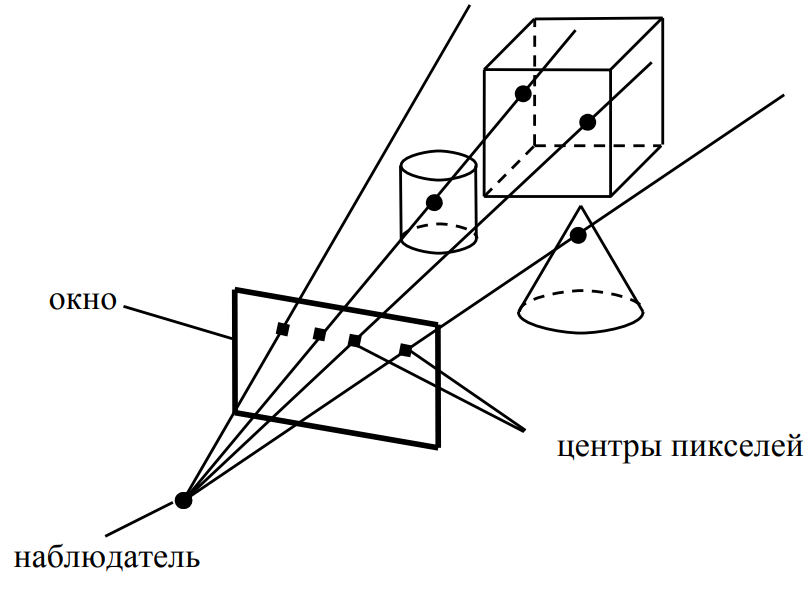
\includegraphics[width=0.8\textwidth]{img/ray_tracing_algorithm_1.png}
    \caption{Трассировка лучей.}
    \label{fig:ray_tracing_algorithm_1}
\end{figure}

Скорость работы алгоритма можно оценить как O(CN), где N – количество граней, C – количество пикселей, так как необходимо луч для каждого пиксела проверить на пересечение с каждой из граней. Для повышения производительности можно воспользоваться когерентностью в пространстве. Грани обычно образуют поверхность объектов, то есть располагаются в пространстве компактными группами. Вокруг таких групп можно описать простые оболочки, например, сферы, и сначала проверять луч на пересечение с оболочкой, и только если он с ней пересекается, искать пересечение с отдельными гранями. Также можно использовать когерентность в картинной плоскости. Если для текущего пиксела была найдена ближайшая грань, то она скорее всего будет ближайшей и для соседних пикселей. Таким образом, для соседнего пиксела можно сначала проверить луч на пересечение с этой гранью. Если оно имеет место, то с остальными гранями достаточно проверять пересечение не всего луча, а только отрезка от наблюдателя до найденной точки пересечения. Это позволит быстрее отбросить грани или описанные тела, находящиеся дальше от наблюдателя, чем эта точка пересечения.~\cite{polski}


\subsubsection{Алгоритм Z-буфера}
\label{subsubsection:Zbuff}

\hspace{1.25cm}
Алгоритм, использующий z-буфер это один из простейших алгоритмов удаления невидимых поверхностей. Впервые он был предложен Кэтмулом. Работает этот алгоритм в пространстве изображения. Идея z-буфера является простым обобщением идеи о буфере кадра. Буфер кадра используется для запоминания атрибутов (интенсивности) каждого пиксела в пространстве изображения, z-буфер - это отдельный буфер глубины, используемый для запоминания координаты z или глубины каждого видимого пиксела в пространстве изображения. В процессе работы глубина или значение z каждого нового пиксела, который нужно занести в буфер кадра, сравнивается с глубиной того пиксела, который уже занесен в z-буфер. Если это сравнение показывает, что новый пиксел расположен впереди пиксела, находящегося в буфере кадра, то новый пиксел заносится в этот буфер и, кроме того, производится корректировка z-буфера новым значением z. Если же сравнение дает противоположный результат, то никаких действий не производится. По сути, алгоритм является поиском по х и у наибольшего значения функции z (х, у).

Главное преимущество алгоритма – его простота. Кроме того, этот алгоритм решает задачу об удалении невидимых поверхностей и делает тривиальной визуализацию пересечений сложных поверхностей. Сцены могут быть любой сложности. Поскольку габариты пространства изображения фиксированы, оценка вычислительной трудоемкости алгоритма не более чем линейна. Поскольку элементы сцены или картинки можно заносить в буфер кадра или в z-буфер в произвольном порядке, их не нужно предварительно сортировать по приоритету глубины. Поэтому экономится вычислительное время, затрачиваемое на сортировку по глубине.

Основной недостаток алгоритма - большой объем требуемой памяти. Если сцена подвергается видовому преобразованию и отсекается до фиксированного диапазона значений координат z, то можно использовать z-буфер с фиксированной точностью. Информацию о глубине нужно обрабатывать с большей точностью, чем координатную информацию на плоскости (х, y); обычно бывает достаточно 20-ти бит. Буфер кадра размером 512´512´24 бит в комбинации с z-буфером размером 512´512´20 бит требует почти 1.5 мегабайт памяти. Однако снижение цен на память делает экономически оправданным создание специализированных запоминающих устройств для z-буфера и связанной с ним аппаратуры.

Альтернативой созданию специальной памяти для z-буфера является использование для этой цели оперативной памяти. Уменьшение требуемой памяти достигается разбиением пространства изображения на 4, 16 или больше квадратов или полос. В предельном варианте можно использовать z-буфер размером в одну строку развертки. Для последнего случая имеется интересный алгоритм построчного сканирования. Поскольку каждый элемент сцены обрабатывается много раз, то сегментирование z-буфера, вообще говоря, приводит к увеличению времени, необходимого для обработки сцены. Однако сортировка на плоскости, позволяющая не обрабатывать все многоугольники в каждом из квадратов или полос, может значительно сократить этот рост.

Другой недостаток алгоритма z-буфера состоит в трудоемкости и высокой стоимости устранения лестничного эффекта, а также реализации эффектов прозрачности и просвечивания. Поскольку алгоритм заносит пикселы в буфер кадра в произвольном порядке, то нелегко получить информацию, необходимую для методов устранения лестничного эффекта, основывающихся на предварительной фильтрации. При реализации эффектов прозрачности и просвечивания пикселы могут заноситься в буфер кадра в некорректном порядке, что ведет к локальным ошибкам. 

Формальное описание алгоритма z-буфера таково:

\begin{enumerate}
\item Заполнить буфер кадра фоновым значением интенсивности или цвета.
\item Заполнить z-буфер минимальным значением z.
\item Преобразовать каждый многоугольник в растровую форму в произвольном порядке.
\item Для каждого Пиксел(x,y) в многоугольнике вычислить его глубину z(x,y).
\item Сравнить глубину z(х,у) со значением Zбуфер(х,у), хранящимся в z-буфере в этой же позиции.
\end{enumerate}

Если z(х,у) > Zбуфер (х,у), то записать атрибут этого многоугольника (интенсивность, цвет и т.п.) в буфер кадра и заменить Zбуфер(х,у) на z(х,у). В противном случае никаких действий не производить.~\cite{zbuffer}

\begin{figure}[H]
    \centering
    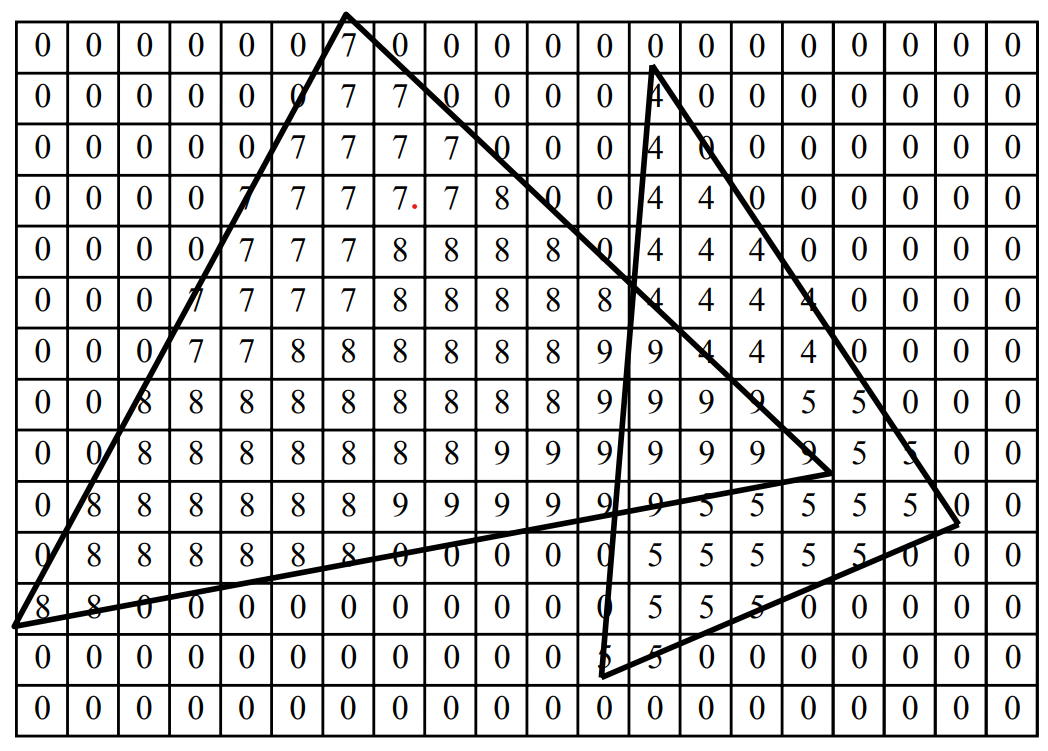
\includegraphics[width=\textwidth]{img/Zbuff_algorithm_1.png}
    \caption{Значения в Z-буфере.}
    \label{fig:Zbuff_algorithm_1}
\end{figure}



\subsubsection{Методы построчного сканирования}

\hspace{1.25cm}
Суть метода построчного сканирования заключается в том,
что через каждую строку пикселей окна проводится плоскость, дающая сечение сцены. При пересечении поверхностей объектов этими плоскостями
образуются некоторые линии, например, при пересечении граней – отрезки, и задача видимости решается для этого набора отрезков (см. рис. ~\ref{fig:string_algorithms_1}). Таким образом, задача определения видимых участков граней в трёхмерном пространстве преобразуется в набор задач определения видимости отрезков на плоскости, которые решаются проще и эффективнее. 

\begin{figure}[H]
    \centering
    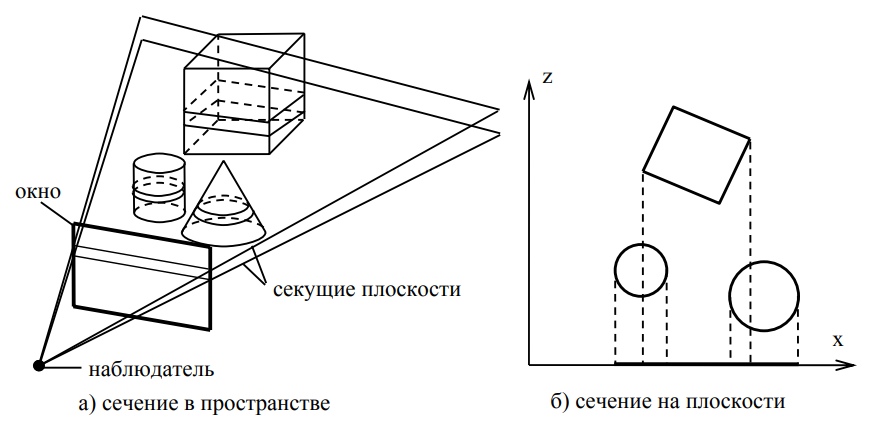
\includegraphics[width=\textwidth]{img/string_algorithms_1.png}
    \caption{Метод построчного сканирования.}
    \label{fig:string_algorithms_1}
\end{figure}

Пересечение плоскости и выпуклой грани является отрезком, на экране он отображается в виде горизонтального отрезка пикселей -- спана.~\cite{polski}


\paragraph{Алгоритм построчного Z-буффера}

\hspace{1.25cm}
Алгоритм работает аналогично обычному Z-буферу (см.~\autoref{subsubsection:Zbuff}),
единственное отличие в том, что вместо двухмерного массива значений
глубины, достаточно одномерного массива размером в строку пикселей.
Каждому пикселу соответствует свой элемент массива, перед рисованием
строки в него заносится максимальное значение глубины, а при рисовании
пикселей спанов их глубина сравнивается с глубиной в Z-буфере и, если
пиксел ближе, он рисуется, а его глубина заносится в Z-буфер. Построчный алгоритм более эффективен, чем полноэкранный, так как Z-буфер требует значительно меньшего объёма памяти и полностью умещается в кэше процессора. Чтобы ещё немного повысить производительность можно воспользоваться когерентностью соседних строк, грани видимые в одной строке, скорее всего, видимы и в соседних. Если рисовать сначала те
грани, которые были видимы в предыдущей строке, а затем все остальные,
то Z-буфер будет сразу заполняться наиболее близкими значениями глубины этих граней, а большинство пикселей остальных граней окажутся
дальше, что позволит сократить количество операций рисования пикселей
и модификации значений глубины в Z-буфере.~\cite{polski}


\paragraph{Алгоритм S-буффера}

\hspace{1.25cm}
S-буфер -- это буфер отрезков видимых наблюдателю (S -- от segment,
отрезок). Отрезки, полученные в результате пересечения граней плоскостью, поочерёдно заносятся в S-буфер. При этом очередной отрезок сначала сравнивается с отрезками буфера. Могут возникнуть следующие случаи:

\begin{itemize}
\item проекции отрезков не пересекаются (см. рис.~\ref{fig:Sbuff_algorithm_1}а), ни один из отрезков не заслоняет другого;
\item новый отрезок может полностью заслонить отрезок буфера (см. рис.~\ref{fig:Sbuff_algorithm_1}б), в этом случае заслонённый отрезок удалятся из буфера;
\item новый отрезок может заслонить часть отрезка буфера (см. рис.~\ref{fig:Sbuff_algorithm_1}в), в этом случае отрезок буфера делится на части и заслонённая часть удаляется из буфера;
\item отрезок из буфера может полностью заслонить новый отрезок (см.
рис.~\ref{fig:Sbuff_algorithm_1}б), в этом случае новый отрезок не виден и не заносится в буфер;
\item отрезок из буфера может заслонить часть нового отрезка (см. рис.~\ref{fig:Sbuff_algorithm_1}в), в этом случае новый отрезок делится на части, заслонённая часть удаляется, а оставшиеся сравниваются с остальными отрезками буфера;
\item отрезки пересекаются (см. рис.~\ref{fig:Sbuff_algorithm_1}г), в этом случае оба отрезка делятся на части, заслонённые части удаляются, оставшиеся части отрезка буфера заносятся обратно в буфер, оставшиеся части нового отрезка сравниваются с остальными отрезками буфера. 
\end{itemize}

\begin{figure}[H]
    \centering
    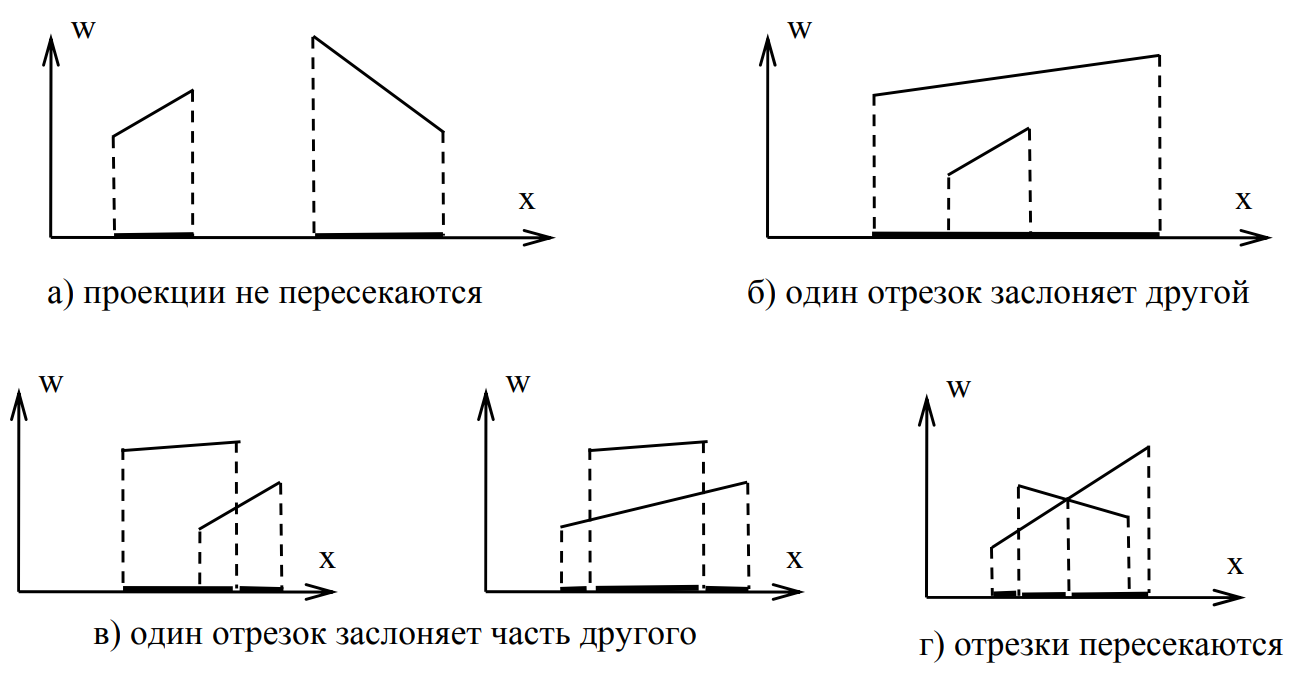
\includegraphics[width=\textwidth]{img/Sbuff_algorithm_1.png}
    \caption{Сравнение двух отрезков.}
    \label{fig:Sbuff_algorithm_1}
\end{figure}

На рисунке~\ref{fig:Sbuff_algorithm_1} ось x – горизонтальная ось окна, ось w – параметр глубины, чем больше w, тем точка ближе к наблюдателю.

Определить, что проекции отрезков не пересекаются можно по условию, что максимальная координата x одного отрезка не превышает минимальную координату x другого. Когда проекции пересекаются, нужно определить, какие части отрезков заслонены (см. рис.~\ref{fig:Sbuff_algorithm_2}). Если отсортировать точки концов отрезков (A, B, C, D) вдоль оси x, то можно выделить три интервала (A-B, B-C, C-D). На первом интервале видна часть отрезка, которому принадлежит точка A, на третьем интервале видна часть отрезка, которому принадлежит точка D.

\begin{figure}[H]
    \centering
    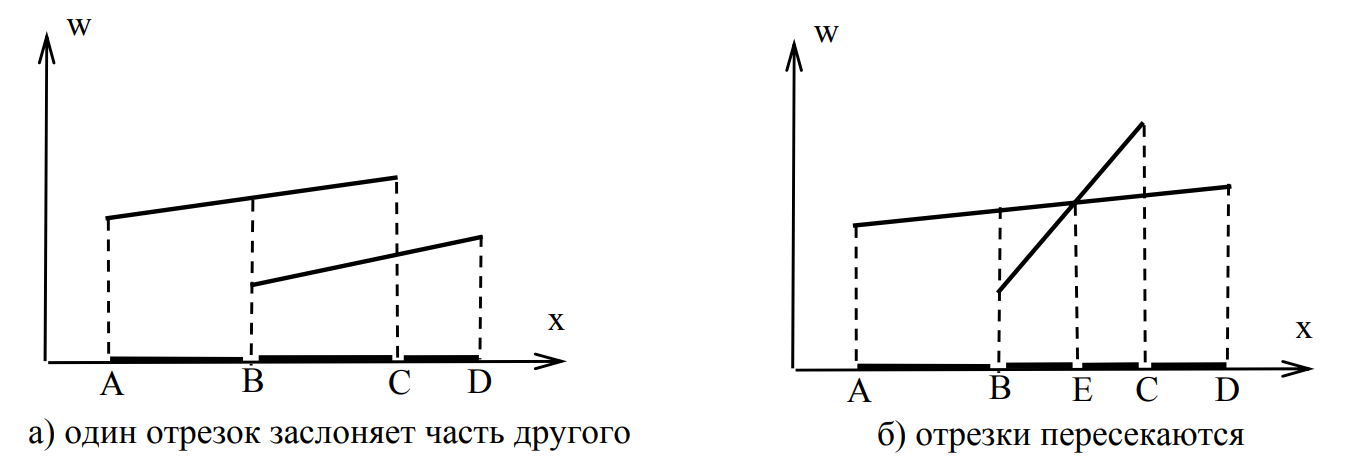
\includegraphics[width=\textwidth]{img/Sbuff_algorithm_2.png}
    \caption{Определение заслонённых частей отрезков.}
    \label{fig:Sbuff_algorithm_2}
\end{figure}

Чтобы определить, какие части видимы на втором интервале, нужно рассчитать глубину точек отрезков на его концах. Для двух точек она известна, так как точки являются концами отрезков, для двух оставшихся
можно рассчитать, используя уравнение прямой:
\[
w = w_1 + (w_2 - w_1) \cdot \frac{x - x_1}{x_2 - x_1},
\]
где $x_1, w_1, x_2, w_2$ – координаты двух концов отрезка, $x, w$ – координаты точки пересечения. Если глубина обеих точек одного отрезка больше, чем у точек второго, то второй отрезок заслонён первым на этом интервале (см. рис.~\ref{fig:Sbuff_algorithm_2}a). Если в начале интервала больше глубина одного отрезка, а в конце – другого, то отрезки пересекаются (см. рис.~\ref{fig:Sbuff_algorithm_2}б). В этом случае необходимо найти точку пересечения отрезков, например, приравняв вышеприведённое уравнение прямой для прямых обоих отрезков. Интервал $B$-$C$ поделится точкой пересечения $E$ на два интервала ($B$-$E$, $E$-$C$). На первом будет виден отрезок, глубина которого в точке $B$ больше, чем у другого, на втором – отрезок, глубина которого в точке $C$ больше, чем у другого.~\cite{polski}

\subsubsection{Выводы}

\hspace{1.25cm}
Таблица~\ref{tab:algorithm_comparison} представляет собой сравнительный анализ алгоритмов удаления невидимых линий по основным критериям, важным для задачи создания и редактирования 3D-сцен. Алгоритмы представлены в столбцах, а критерии их оценки — в строках. 

\textbf{Обозначения алгоритмов:}
\begin{itemize}
    \item \textbf{ПГ} — Алгоритм плавающего горизонта.
    \item \textbf{Роб} — Алгоритм Робертса.
    \item \textbf{Вар} — Алгоритм Варнака.
    \item \textbf{В-А} — Алгоритм Вейлера-Азертона.
    \item \textbf{Худ} — Алгоритм художника.
    \item \textbf{ТЛ} — Алгоритм трассировки лучей.
    \item \textbf{Z-Б} — Алгоритм Z-буфера.
    \item \textbf{ПС} — Методы построчного сканирования.
\end{itemize}

\textbf{Обозначения уровней оценки:}
\begin{itemize}
    \item \textbf{В} — Высокий уровень.
    \item \textbf{С} — Средний уровень.
    \item \textbf{Н} — Низкий уровень.
    \item \textbf{ОВ} — Очень высокий уровень.
    \item \textbf{Огр} — Ограниченная функциональность.
\end{itemize}

Таблица позволяет легко сравнить алгоритмы по таким критериям, как простота реализации, скорость работы, точность результата, объём используемой памяти и уровень интерактивности. Данные сокращения обеспечивают компактное представление информации, сохраняя при этом её содержательность.


\begin{table}[H]
\centering
\renewcommand{\arraystretch}{1.5}
\setlength{\tabcolsep}{10pt}
\begin{tabular}{|c|c|c|c|c|c|c|>{\columncolor{blue!10}}c|c|}
\hline
\textbf{Критерий}  & \textbf{ПГ} & \textbf{Роб} & \textbf{Вар} & \textbf{В-А} & \textbf{Худ} & \textbf{ТЛ} & \textbf{Z-Б} & \textbf{ПС} \\ \hline
\textbf{Простота}  & С           & Н            & С            & Н            & В            & Н           & В           & С           \\ \hline
\textbf{Скорость}  & В           & С            & С            & Н            & В            & Н           & Н           & В           \\ \hline
\textbf{Точность}  & С           & В            & В            & ОВ           & С            & ОВ          & В           & С           \\ \hline
\textbf{Память}    & Н           & Н            & Н            & С            & Н            & В           & Н          & Н           \\ \hline
\textbf{Интерактивность} & Н    & Н            & Огр          & Огр          & В            & Огр         & С           & В           \\ \hline
\end{tabular}
\caption{Сравнение алгоритмов удаления невидимых линий по критериям}
\label{tab:algorithm_comparison}
\end{table}

Алгоритм Z-буфера выбран для задачи построения цифровой модели помещения по следующим причинам:

\begin{enumerate}
\item Точность: Z-буфер позволяет точно определять видимость объектов, так как каждый пиксель имеет соответствующую глубину, что важно для сцены, состоящей из параллелепипедов.

\item Скорость: Несмотря на то, что Z-буфер может требовать значительных вычислительных ресурсов для сложных сцен, он остаётся достаточно быстрым для большинства случаев. Однако для сложных сцен с высоким разрешением может потребоваться больше времени на перерасчёт и больше памяти из-за хранения матрицы глубины для каждого пикселя.

\item Память: Хотя Z-буфер требует много памяти для хранения данных о глубине, это компенсируется его простотой и высокой точностью. Однако в интерактивных приложениях, где сцена изменяется динамически, перерасчёт для каждого пикселя может быть медленным.
\end{enumerate}

Таким образом, Z-буфер подходит для решения задачи, но требует оптимизаций, если сцена будет сложной или с большим количеством объектов.




\subsection{Алгоритмы отрисовки теней}

%\hspace{1.25cm}

\subsubsection{Введение}

\hspace{1.25cm}
Тени являются неотъемлемой частью реалистичных изображений в компьютерной графике. Они помогают передать пространственные соотношения между объектами сцены, добавляют глубину и реализм визуализации. Существует множество методов отрисовки теней, которые варьируются по сложности и требуемым вычислительным ресурсам. В связи с выбором алгоритма Z-буфера для удаления невидимых линий и плоскостей, удобно использовать его и для алгоритма построения теней. Такой подход позволяет сохранить простоту структуры программы, исключить сложности при интеграции двух разных методов и, как следствие, сократить время, необходимое на отладку алгоритма.


\subsubsection{Принципы работы Z-буфера}

\hspace{1.25cm}
Алгоритм Z-буфера основывается на хранении информации о глубине объектов сцены для каждого пикселя экрана. При расчёте теней алгоритм проходит два этапа:

\begin{enumerate}
    \item \textbf{Первый проход:} Сцена анализируется с позиции источника света. Вычисляются точки, видимые со стороны источника, и их глубины заносятся в теневой Z-буфер.
    \item \textbf{Второй проход:} Сцена визуализируется с позиции наблюдателя. Для каждого пикселя проверяется, находится ли он в тени, путём сравнения его координат с данными теневого Z-буфера.
\end{enumerate}


Преимущества Z-буфера для отрисовки теней:

\begin{itemize}
    \item Универсальность: метод подходит для сцен любой сложности, включая динамические сцены с движущимися объектами и источниками света.
    \item Реализация в реальном времени: алгоритм хорошо масштабируется на современных графических процессорах, обеспечивая приемлемую скорость работы.
    \item Простота интеграции: Z-буфер легко адаптируется для построения теней, поскольку он изначально используется для удаления невидимых поверхностей.
\end{itemize}

Ограничения метода:

\begin{itemize}
    \item Артефакты на границах теней: из-за дискретизации возможны погрешности, такие как акне (z-fighting) или ступенчатые края.
    \item Сложность мягких теней: алгоритм изначально рассчитан на жёсткие тени. Реализация эффектов мягкости требует дополнительных вычислений.
\end{itemize}


\subsubsection{Выводы}

\hspace{1.25cm}
Алгоритм Z-буфера является эффективным выбором для построения теней в условиях, когда требуется высокая скорость и приемлемое качество визуализации. Несмотря на некоторые ограничения, он остаётся стандартным методом, широко применяемым в компьютерной графике благодаря простоте и универсальности.~\cite{romanyuk_kurinnyy}




\subsection{Алгоритмы затенения}

\subsubsection{Введение}

\hspace{1.25cm}
В компьютерной графике широко используются алгоритмы затенения для наложения освещения на объекты сцены. Рассмотрим две наиболее популярные модели: затенения по Гуро (Gouraud shading) и затенения по Фонгу (Phong shading).

\subsubsection{Затенение по Гуро}

\hspace{1.25cm}
Модель затенения по Гуро предполагает линейную интерполяцию цвета между вершинами полигона. Это требует, чтобы нормали были заданы в вершинах, так как цвет рассчитывается на основе нормалей. Преимущества и недостатки модели:

\begin{itemize}
    \item \textbf{Преимущества:}
    \begin{itemize}
        \item Высокая скорость работы: дорогостоящие расчёты освещения производятся только в вершинах.
        \item Легко оптимизируется благодаря линейной интерполяции.
    \end{itemize}
    \item \textbf{Недостатки:}
    \begin{itemize}
        \item Потеря бликов на поверхности при низкой детализации модели.
        \item Размытые отражения, особенно заметные на крупных полигонах.
    \end{itemize}
\end{itemize}

\begin{figure}[h!]
    \centering
    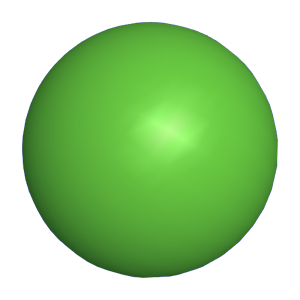
\includegraphics[width=0.4\textwidth]{img/gouraud1.png}
    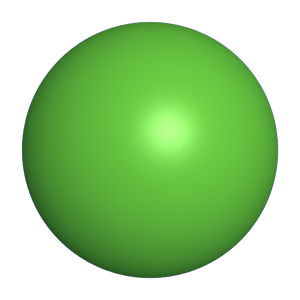
\includegraphics[width=0.4\textwidth]{img/gouraud2.png}
    \caption{Сфера с затенением по Гуро: около 2000 (слева) и 32000 треугольников (справа).}
\end{figure}

\subsubsection{Затенение по Фонгу}

\hspace{1.25cm}
Затенение по Фонгу работает иначе: между вершинами интерполируется не цвет, а нормаль, а освещение рассчитывается для каждого пикселя. Это позволяет добиться более высокой визуальной точности:

\begin{itemize}
    \item \textbf{Преимущества:}
    \begin{itemize}
        \item Качественное изображение без смазывания бликов.
        \item Высокая степень реализма благодаря попиксельному расчёту освещения.
    \end{itemize}
    \item \textbf{Недостатки:}
    \begin{itemize}
        \item Высокие вычислительные затраты, особенно для сцен с высоким разрешением.
    \end{itemize}
\end{itemize}

\begin{figure}[h!]
    \centering
    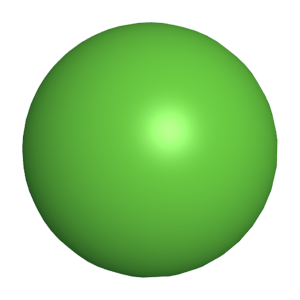
\includegraphics[width=0.4\textwidth]{img/phong1.png}
    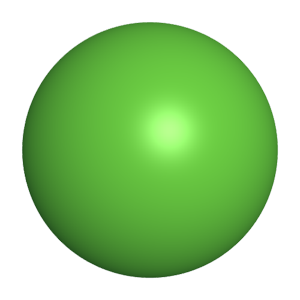
\includegraphics[width=0.4\textwidth]{img/phong2.png}
    \caption{Сфера с затенением по Фонгу: около 2000 (слева) и 32000 треугольников (справа).}
\end{figure}

\subsubsection{Выводы}

\hspace{1.25cm}
Модель затенения по Гуро обладает достаточной скоростью для многих задач, однако затенение по Фонгу обеспечивает значительно более реалистичное изображение, особенно для сложных сцен. Благодаря современным графическим процессорам затенение по Фонгу стало стандартом в игровой индустрии.~\cite{compgraphics}


\newpage